\section{i numeri reali}
\subsection{costruzione dei numeri reali}
\label{sec:costruzione_reali}

La proprietà che manca al campo $\QQ$ dei numeri razionali 
è la \emph{continuità}. 
Non è sufficiente aggiungere una nuova operazione, ma bisogna 
fare in modo che ogni coppia di insiemi separati 
abbia elemento di separazione 
(si veda la definizione~\ref{def:ordinamento_continuo})
ovvero bisogna che ogni insieme non vuoto e superiormente 
limitato abbia estremo superiore.

Possiamo allora definire l'insieme dei \emph{numeri reali}
così:
\index{reali!insieme dei}%
\index{numero!reale}%
\index{insieme!numeri reali}%
\[
\RR = \ENCLOSE{A \in \mathcal P(\QQ)\colon A\neq \emptyset, \text{ $A$ superiormente 
limitato}}/\sim
\]
dove poniamo $A\sim B$ 
se $A$ e $B$ hanno gli stessi maggioranti, ovvero
se per ogni $q\in \QQ$ si ha $q\ge A \iff q\ge B$.
L'idea di questa definizione è che i numeri reali 
possono essere identificati dalle loro approssimazioni 
per difetto tramite numeri razionali. 
Diverse approssimazioni, però, possono rappresentare 
lo stesso numero reale.

\begin{exercise}
  Si mostri che si ha $A \sim B \sim C$
  per i seguenti insiemi:
  \[
  A = \ENCLOSE{1}, \qquad 
  B = \ENCLOSE{x\in \QQ\colon x<1}, \qquad
  C = \ENCLOSE{\frac{n}{n+1}\colon n\in \NN}.
  \]
\end{exercise}

\begin{exercise}
  Si mostri che si ha $A\sim B$ se
  \[
  A = \ENCLOSE{x\in \QQ\colon x^2<2}, \qquad
  B = \ENCLOSE{\frac{n}{10^k}\colon n\in \NN, k\in \NN, n^2 \le 2\cdot 100^k < (n+1)^2}.  
  \]
  Verificare che 
  \[
    B \supset \ENCLOSE{
      1,\frac{14}{10},\frac{141}{100},\frac{1414}{1000},
      \frac{14142}{10000}}.
  \]
\end{exercise}

Vogliamo ora definire su $\RR$ una struttura di gruppo ordinato.

L'ordinamento di $\QQ$ può essere facilmente esteso a $\RR$
definendo $\Enclose{A}_\sim \le \Enclose{B}_\sim$ se ogni maggiorante di $B$ 
è anche maggiorante di $A$. Questa definizione non dipende dalla scelta 
di $A$ e $B$ nella loro classe di equivalenza perché all'interno della classe di 
equivalenza l'insieme dei maggioranti 
non cambia.

Per l'addizione, dati $A,B$ sottoinsiemi non vuoti e superiormente limitati di $\QQ$, 
definiamo 
\[
  \Enclose{A}_\sim+\Enclose{B}_\sim
  = \Enclose{A+B}_\sim
  \qquad\text{dove $A+B = \ENCLOSE{a+b\colon a \in A, b \in B}$.}
\]
Chiaramente $A+B$ è non vuoto e superiormente limitato
inoltre non è difficile dimostarare che 
se $A\sim A'$ e $B\sim B'$ si ha $A+B\sim A'+B'$.

\begin{theorem}
  \label{th:reali_gruppo_continuo}%
Con l'addizione e l'ordinamento appena definiti, 
$\RR$ risulta essere un gruppo additivo totalmente ordinato, denso e continuo.
(definizioni~\ref{def:ordinamento_denso}, \ref{def:gruppo_ordinato}, \ref{def:ordinamento_continuo}).
\end{theorem}
\begin{proof}
  Chiaramente $x\le x$, se $x\le y$ e $y\le x$ si ha $x=y$ 
  e se $x\le y$, $y\le z$ si ha $x\le z$: dunque $\le$ è un ordinamento su $\RR$.
  E' inoltre un ordinamento totale perché dati $x=\Enclose{A}_\sim$ e 
  $y=\Enclose{B}_\sim$ se $x\neq y$ significa che l'insieme dei maggioranti 
  di $A$ è diverso dall'insieme dei maggioranti di $B$. 
  Supponiamo allora che esista $q$ che è maggiorante di $A$ 
  ma non maggiorante di $B$ (se succede il viceversa basta scambiare $A$ e $B$).
  In tal caso $B\ge A$ in quanto ogni maggiorante di $B$ deve essere maggiore 
  di $q$ e quindi deve essere anche un maggiorante di $A$ da cui $x\le y$. 
  
  Ovviamente l'addizione su $\RR$ è associativa e commutativa in quanto 
  queste proprietà valgono su $\QQ$ e di conseguenza sui suoi sottoinsiemi:
  $(A+B)+C = \{ a+b+c\colon a\in A, b\in B, c\in C\} = A + (B+C)$ e 
  $A+B = \{a+b\colon a\in A, b\in B\} = B+A$.
  Visto che $A+\ENCLOSE{0} = A$ notiamo anche che $\Enclose{\ENCLOSE{0}}_\sim$ 
  è elemento neutro dell'addizione.
  
  Dato $A\in \mathcal R$ denotiamo con $A'$ l'insieme dei maggioranti di $A$.
  Vogliamo dimostrare che $A$ e $A'$ contengono punti arbitrariamente vicini:
  \begin{equation}\label{eq:48023775}
  \forall \eps\in\QQ\colon (\eps >0 \implies \exists a \in A\colon \exists b\in A'\colon
  b-a < \eps).
  \end{equation}
  Per fare ciò prendiamo qualunque $c\in A$ 
  e prendiamo qualunque $q\in A'$ 
  ($A\neq \emptyset$ e visto che $A$ è superiormente limitato, 
  $A'\neq \emptyset$).
  L'insieme $I=\ENCLOSE{n\in \NN \colon c+n\eps\in A'}$
  non è vuoto in quanto se $n>\frac{q-c}\eps$ si ha $c+n\eps>q$ ed essendo $q$ 
  un maggiorante di $A$ anche $c+n\eps$ lo è.
  Dunque per il buon ordinamento di $\NN$ (teorema~\ref{th:buon_ordinamento})
  l'insieme $I$ ha minimo, che chiamiamo $k$.
  Se $k=0$ significa che $c\in A'$ e posto $a=b=c$ si ottiene 
  che \eqref{eq:48023775} è banalmente verificata.
  Altrimenti prendiamo $b=c+k\eps$.
  Per la scelta di $k$ sappiamo che $b\in A'$ e $c+(k-1)\eps$ non è un maggiorante di 
  $A$. 
  Ma allora esiste $a\in A$ tale che $a>c+(k-1)\eps$ da cui 
  $b-a < \eps$ e \eqref{eq:48023775} è ancora verificata.
  
  Possiamo ora osservare che posto $B=-A' = \{-x\in \QQ \colon x$ maggiorante di $A\}$
  si ha $(A+B)\sim\ENCLOSE{0}$. 
  I maggioranti di $\ENCLOSE{0}$ sono i $q\in \QQ$ con $q\ge 0$, 
  vogliamo dimostrare che anche $A+B$ ha gli stessi maggioranti.
  Ma se $a\in A$ e $b\in B$ risulta che $-b\ge a$ ovvero $a+b\le 0$ 
  dunque $0$ è un maggiorante di $A+B$ e qualunque $q\ge 0$ lo è a maggior ragione.
  Se invece $q<0$ per la proprietà \eqref{eq:48023775} esistono $a\in A$ 
  e $-b\in A'$ (cioè $b\in B$) tali che $(-b)-a<-q$ cioè $a+b>q$. Dunque 
  $q<0$ non è un maggiorante di $A+B$ e concludiamo che $A+B\sim\ENCLOSE{0}$.
  
  Questo dimostra che dato qualunque $x\in \RR$ se $x=\Enclose{A}_\sim$
  posto $y=\Enclose{-A'}$ si ha $x+y=\Enclose{0}_\sim$.
  Dunque ogni $x\in \RR$ ha opposto $y$ che denoteremo 
  con $y=-x$.

  L'ordinamento è compatibile con l'addizione perché se $\Enclose{A}_\sim 
  \le \Enclose{B}_\sim$ e $A,B,C\in \mathcal R$ 
  allora se $q$ è maggiorante di $B+C$ per ogni $c\in C$ si ha che $q-c$ 
  è maggiorante di $B$ e dunque $q-c$ è anche maggiorante di $A$.
  Ma allora $q$ è maggiorante di $A+C$. Dunque se $x\le y$ e $x,y,z\in \RR$ 
  si ha $x+z\le y+z$ e $\RR$ è un gruppo ordinato.
  
  L'ordinamento di $\RR$ è denso (definizione~\ref{def:ordinamento_denso}). 
  Infatti se $x<y$ posto $y-x=\Enclose{A}_\sim$ 
  sappiamo che ogni maggiorante di $A$ è maggiore o uguale a $0$.
  Ma se ogni numero positivo fosse maggiorante di $A$ avremmo $A\sim\ENCLOSE 0$
  che non è possibile in quanto $x\neq y$. Dunque esiste $q>0$ 
  che non è maggiorante di $A$. 
  Ma allora $y-x \ge \Enclose{\ENCLOSE q}_\sim > \Enclose{\ENCLOSE{\frac q 2}}_\sim = \eps > 0$
  da cui $x<x+\eps<y$.
  
  Dimostriamo ora che l'ordinamento è continuo.
  Siano dati $\mathcal A$ e $\mathcal B$ sottoinsiemi non vuoti di $\RR$ 
  con $\mathcal A\le \mathcal B$. 
  Possiamo definire
  \begin{align*}
    C & = \bigcup\ENCLOSE{A\in \mathcal P(\QQ)\colon \Enclose{A}_\sim \in \mathcal A} \\
      &= \ENCLOSE{q\in \QQ\colon \exists A\colon 
      (\Enclose{A}_\sim \in \mathcal A) \land (q\in A)}.
  \end{align*}
  Preso qualunque $a=\Enclose{A}_\sim \in \mathcal A$ risulta 
  ovviamente $A\subset C$. In particolare $C$ non è vuoto.
  Mentre se $b=\Enclose{B}_\sim \in \mathcal B$ 
  preso qualunque $q\in C$ si ha $q\in A$ per un qualche $A$ tale che 
  $\Enclose{A}_\sim = a\in \mathcal A$.
  Ma visto che $a\le b$, ogni maggiorante di $B$ è anche maggiorante di $A$.
  In particolare preso un qualunque $r$ maggiorante di $B$
  risulta che $r$ è un maggiorante di $C$.
  Allora $C$ è non vuoto e superiormente limitato 
  e posto $c=\Enclose{C}_\sim$ 
  risulta che ogni maggiorante di $C$ è maggiorante di 
  ogni $A$ con $\Enclose{A}_\sim \in \mathcal A$ mentre 
  ogni maggiorante di un qualunque $B$ con $\Enclose{B}_\sim\in \mathcal B$ 
  è anche un maggiorante di $C$.
  Questo significa che $c\ge a$ per ogni $a\in A$ 
  e $b\ge c$ per ogni $b\in B$: la dimostrazione è conclusa.
\end{proof}

Ad ogni $q\in \QQ$ si può associare l'elemento $\Enclose{\ENCLOSE q}_\sim$ 
di $\RR$. Ovviamente se $q\neq s$ in $\QQ$ allora $\ENCLOSE{q}$ 
ed $\ENCLOSE{s}$ non hanno gli stessi maggioranti e quindi si ottengono 
elementi distinti di $\RR$. 
Non solo, dati $x<y$ in $\RR$ possiamo sempre trovare $q\in \QQ$ tale che 
$x < \Enclose{\ENCLOSE q}_\sim < y$. 
Se $x=\Enclose{A}_\sim$ e $y=\Enclose{B}_\sim$
basta infatti prendere un maggiorante $m\in \QQ$ di $A$ che non sia maggiorante di $B$
e un elemento $M>m$ di $B$ e scegliere $q$ tale che $m<q<M$.

Identificando $q$ con $\Enclose{\ENCLOSE q}_\sim$ 
possiamo quindi pensare che sia $\QQ \subset \RR$ e risulta così che $\QQ$ è denso in 
$\RR$ e, di conseguenza, $\RR$ è esso stesso denso.

Così come abbiamo esteso l'addizione da $\QQ$ a $\RR$ possiamo
si potrebbe facilmente estendere anche l'operazione di moltiplicazione.
% Dovremo solo fare attenzione che la moltiplicazione per un numero negativo 
% inverte l'ordinamento e quindi scambia i maggioranti con i minoranti.
% 
% Dato $x\in \RR$ e $y\in \RR$, $y \ge 0$, si avrà $x=[A]_\sim$ e $y=[B]_\sim$
% per qualche $A,B$ sottoinsiemi non vuoti e superiormente limitati di $\QQ$.
% Potremo allora definire:
% \[
%   y\cdot x = [A\cdot B]_\sim
% \]  
% dove $A\cdot B$ è l'insieme di tutti i prodotti $a\cdot b$ con $a\in A$ 
% e $b\in B$.
Non ci servirà però definire ora la moltiplicazione, la potremo ottenere 
più avanti grazie ad una costruzione più generale (teorema~\ref{th:moltiplicazione_reali})

\subsection{unicità dei numeri reali}

Nel capitolo precedente abbiamo costruito un insieme $\RR$ 
che risulta essere un gruppo additivo totalmente ordinato 
denso e continuo. 
In questo capitolo vogliamo dimostrare (teorema~\ref{th:isomorfismo})
che $\RR$ è sostanzialmente l'unico gruppo che soddisfa 
tali proprietà, nel senso che ogni gruppo additivo totalmente ordinato 
denso continuo e non banale, è isomorfo a $\RR$.

% Esistono dei gruppi additivi che estendono $\RR$, ma nessuna 
% estensione mantiene tutte le proprietà dell'ordinamento di $\RR$.
% I numeri \emph{complessi} (li vedremo tra poco), 
% e i \emph{quaternioni}, ad esempio, non sono totalmente ordinati.
% I numeri \emph{iperreali} di Robinson, alla base dell'analisi non standard, 
% non soddisfano la proprietà di continuità dell'ordinamento. 
% Lo stesso vale per i numeri \emph{surreali} introdotto da Conway.

Vogliamo quindi considerare un generico gruppo additivo 
denso e continuo $R$. 
Supporremo anche che $R$ non sia banale, cioè che il gruppo non
consista solamente dell'elemento neutro: $R\neq \ENCLOSE{0}$.

In effetti le proprietà di $R$ corrispondono esattamente 
alle proprietà che ci aspettiamo debba avere una retta geometrica:
l'ordinamento corrisponde alla proprietà che ogni punto 
della retta divide la retta in due parti e che fissati due punti 
si possono identificare i punti intermedi.
L'operazione di addizione corrisponde alla possibilità 
di effettuare traslazioni lungo la retta.

% Intuitivamente si può ottenere l'insieme $\RR$ dei numeri reali
% a partire da una retta geometrica 
% con lo stesso procedimento con cui si costruisce un righello.
% Iniziamo col segnare
% sulla retta un punto di riferimento che chiamiamo $0$, 
% dopodiché osserviamo che
% il punto $0$ (come ogni altro punto) divide la retta in due parti. In modo arbitrario
% chiamiamo positivi i punti che si trovano da una parte e negativi i punti che
% si trovano dall'altra parte. Sulla semiretta dei numeri positivi scegliamo, arbitrariamente,
% un punto $1$. Il segmento compreso tra i punti $0$ e $1$ sarà la nostra unità di
% misura.
% L'addizione potrebbe essere definita utilizzando i movimenti rigidi.
% Traslando il punto $1$ di una unità alla volta si ottengono, per iterazione, tutti i numeri naturali.
% Traslando all'indietro si ottengono i numeri interi negativi. 
% Assumendo che tra due punti qualunque esistano sempre punti intermedi (divisibilità) e
% assumendo che suddividendo la retta in due parti esista sempre un punto di 
% suddivisione (continuità) mostreremo come si può suddividere 
% ogni segmento in $n$ parti uguali per ogni numero naturale $n$. 
% In tal modo potremo ritrovare i numeri razionali e la moltiplicazione per un numero razionale.
% Con una estensione crescente riusciremo quindi a definire la moltiplicazione 
% tra numeri reali. 
% Osserveremo poi che la struttura moltiplicativa dei numeri reali positivi soddisfa 
% gli stessi assiomi della struttura additiva dei reali e che quindi la costruzione fatta 
% per costruire la moltiplicazione si potrà ripetere identica per costruire l'elevamento a potenza.

\begin{theorem}[proprietà archimedea]
  \label{th:archimede}%
  \mymark{**}%
  \mymargin{proprietà archimedea}%
  \index{proprietà!archimedea}%
  \mynote{Questo teorema ci dice che il gruppo $R$ 
  non contiene né elementi \emph{infiniti} (cioè più grandi di qualunque 
  multiplo di un numero positivo $x$) 
  né elementi \emph{infinitesimi} (cioè più piccoli 
  di qualunque frazione $\frac{x}{n}$ con $x>0$ e $n\in \NN$).
  Dunque le quantità infinitesime
  utilizzate da Newton e Leibniz per definire derivate e 
  integrali, non sono giustificabili all'interno 
  di un gruppo totalmente ordinato denso e continuo.
  E' però possibile definire un gruppo totalmente ordinato 
  denso ma non continuo in cui esistono quantità infinite e infinitesime:
  è quello che viene fatto nella \emph{analisi non-standard}.
  \index{analisi non standard}%
  }
    Sia $R$ un gruppo totalmente ordinato, denso e continuo.
  Allora per ogni $x,y\in R$, $x>0$, $y>0$ 
  esiste $n\in \NN$ tale che $n\cdot x > y$.
\end{theorem}
%
\begin{proof}
\mymark{*}%
Fissato $x>0$ consideriamo gli insiemi:
\[
A = \NN\cdot x = \ENCLOSE{n\cdot x\colon n\in \NN},
B = \ENCLOSE{b\in R\colon \forall n\in\NN\colon n \cdot x \le b }.
\]
Per definizione $A\le B$ e $A$ è diverso dal vuoto.
Se per assurdo il teorema fosse falso, si avrebbe $y\in B$ 
e quindi anche $B$ sarebbe non vuoto.
Dunque per la continuità dell'ordinamento dovrebbe esistere 
un elemento di separazione $s\in R$ tale che $A\le s\le B$.
Visto che $s-x<s$ e $s\le B$,
sappiamo che $s-x \not \in B$.
Dunque esiste $n\in \NN$ tale che $n\cdot x > s-x$
ma allora $(n+1)\cdot x > s-x+x=s$. 
Ma questo è assurdo perché $(n+1)\cdot x\in A$ e $s\ge A$.
%
%%% dimostrazione col SUP
%  Fissati $x,y\in R$, $x,y>0$ consideriamo l'insieme 
%  \[
%     A = \NN \cdot y = \ENCLOSE{n\cdot y\colon n\in \NN}.
%  \]
%  Basta dimostrare che $A$ non è superiormente limitato perché 
%  in tal caso dato $x\in \RR$ esisterebbe $n\in \NN$ per cui $n\cdot y> x$.
%
%  Chiaramente $A$ non è vuoto in quanto $0\in A$ dunque se $A$ 
%  per assurdo fosse superiormente limitato esisterebbe 
%  $m=\sup A$, $m\in R$. 
%  Siccome $m$ è il minimo dei maggioranti di $A$
%  e $m-y$ è più piccolo di $m$, allora $m-y$ non è un maggiorante. 
%  Dunque deve esistere $n\in \NN$ tale che $ny>m-y$.
%  Ma allora $(n+1)y = ny + y > m$ ed essendo $n+1\in \NN$ troviamo che $m$
%  non poteva essere un maggiorante di $A$: assurdo.
\end{proof}

Se $n\cdot x = y$ e $n\neq 0$ scriveremo $x=\frac y n$. 
Affinché questa definizione sia univoca bisogna però verificare che 
se $n\cdot x = n\cdot x'$ allora $x=x'$.
Infatti si ha 
\[
  0 = n\cdot x - n\cdot x' = n\cdot (x-x')
\]
e se $n\neq 0$ si conclude $x-x'=0$ ovvero $x=x'$.

Il seguente teorema ci permette di dimostrare che la divisione per $n\neq 0$ 
si può sempre fare.
Si faccia presente che se interpretiamo questo teorema su un 
gruppo moltiplicativo, invece che additivo, il risultato
appare meno banale perché 
stiamo dimostrando l'esistenza della radice $n$-esima.

\begin{theorem}[divisibilità]
\label{th:divisibile}%
Se $R$ è un gruppo additivo totalmente ordinato, denso e continuo
allora per ogni $y\in R$, e per ogni $n\in \NN$, $n\neq 0$ 
esiste $x\in R$ tale che $n\cdot x = y$.
\end{theorem}
%
Per dimostrare il teorema ci servirà il seguente.
%
\begin{lemma}[esistenza di numeri piccoli]
  \label{lm:numeri_piccoli}%
Sia $R$ un gruppo additivo totalmente ordinato e denso.
Per ogni $y\in R$, $y>0$ ed ogni $n\in \NN$ esiste $x\in R$, 
$x>0$ tale che $nx\le y$.
\end{lemma}
%
\begin{proof}
Vogliamo innanzitutto dimostrare che 
\begin{equation}\label{eq:41095633}
  \forall y>0 \colon \exists x>0 \colon x+x \le y.
\end{equation}
Per la proprietà di densità sappiamo che esiste $z$ tale che 
$0<z<y$. 
Prendiamo $w=y-z$. Se $w\le z$ allora $w+w\le w+z=y$ e possiamo prendere $x=w$.
Altrimenti $z+z < w+z = y$ e possiamo prendere $x=z$.
%% Attenzione: la dimostrazione è delicata se il gruppo non è commutativo: bisogna 
%% fare attenzione all'ordine degli addendi! 

Consideriamo ora l'insieme $M$ dei numeri naturali che 
soddisfano il teorema:
\[
  M \defeq \ENCLOSE{m\in \NN\colon \exists x>0\colon mx\le y}.
\]
Basterà dimostrare che $M=\NN$, lo possiamo fare per induzione.
Ovviamente $0\in M$ e $1\in M$ perché basta scegliere $x=y$.
Supponendo ora che $m\in M$, $m\ge 1$, basterà dimostrare che anche $m+1\in M$.
Se $m\in \NN$ esiste $z>0$ tale che $m\cdot z\le y$.
Per la proprietà~\eqref{eq:41095633} esiste $x>0$ tale che $2\cdot x\le z$.
Allora 
\[
  (m+1)\cdot x 
  \le (m+m)\cdot x 
  = m\cdot(2\cdot x)
  \le m\cdot z \le y
\]
e dunque $m+1\in M$ come volevamo dimostrare.
\end{proof}
%
\begin{proof}[Dimostrazione del teorema~\ref{th:divisibile}]
  Dobbiamo dimostrare che per ogni $y\in R$ e per ogni $n\in \NN$, $n\neq 0$
  esiste $x\in R$ tale che $n\cdot x=y$.
  Per fissare le idee supponiamo che sia $y>0$: il caso $y=0$ è banale 
  e se $y<0$ basterà applicare il risultato all'opposto $-y$.
  
  Fissati $n\in \NN$, $n\neq 0$ e $y\in R$, $y>0$ 
  consideriamo allora gli insiemi:
  \begin{align*}
    A &= \ENCLOSE{a\in R\colon n\cdot a\le y},\\
    B &= \ENCLOSE{b\in R\colon n\cdot b\ge y}.
  \end{align*}
  Chiaramente $0\in A$ e $y\in B$ quindi $A$ e $B$ non sono vuoti.
  Inoltre si ha $a\le b$ per ogni $a\in A$ e $b\in B$ 
  perché se fosse $b < a$ si avrebbe $nb < na$ 
  (necessariamente $b>0$) che 
  è assurdo essendo $na \le y \le nb$.
  
  Dunque $A\le B$ sono separati e non vuoti e per l'ipotesi di continuità di $R$ 
  possiamo dedurre che esiste $x$ elemento di separazione: $A\le x \le B$.
  Il nostro obiettivo è dimostrare che $n\cdot x=y$.

  Se fosse $n\cdot x > y$ per il lemma~\ref{lm:numeri_piccoli} dovrebbe 
  esistere $\eps>0$ tale che $n\cdot \eps < n\cdot x - y$.
  Per $k$ abbastanza grande si avrà $(k+1)\eps > x$ e quindi prendendo 
  il minimo $k\in \NN$ con tale proprietà si avrà
  \mynote{Il teorema~\ref{th:buon_ordinamento} garantisce 
  che ogni insieme non vuoto di numeri naturali ha minimo} 
  $k\cdot \eps < x \le (k+1)\cdot \eps$.
  Ma allora 
  \mynote{Non abbiamo supposto che l'addizione sia commutativa,
  ma sfruttiamo il fatto che i multipli di uno stesso numero 
  $\eps$ commutano tra loro.}
  \[
    n\cdot \eps + n\cdot k\cdot \eps
    = n(k+1)\cdot \eps 
    \ge n\cdot x 
    > n\cdot \eps + y 
  \]
  cioè $n\cdot k\cdot \eps > y$ da cui
  $k\cdot \eps \in B$. 
  Ma $k\cdot\eps < x \le B$ e quindi abbiamo un assurdo.

  D'altra parte se fosse $n\cdot x < y$ per il lemma~\ref{lm:numeri_piccoli}
  dovrebbe esistere $\eps>0$ tale che $n\cdot \eps < y-n\cdot x$.
  Allora, analogamente a prima, esiste $k\in\NN$ tale che 
  $k\cdot \eps \le x < (k+1)\cdot \eps$ e quindi
  \[
    n\cdot (k+1) \cdot \eps 
    = n\cdot \eps + n \cdot k \cdot \eps 
    < y - n\cdot x + n\cdot x 
    =y.  
  \]
  Dunque $(k+1)\cdot \eps \in A$ e questo è assurdo perché 
  $(k+1)\cdot \eps > x \ge A$.

  Possiamo quindi concludere che $n\cdot x = y$, come volevamo dimostrare.
\end{proof}
%

\subsection{teorema di isomorfismo}
\label{sec:isomorfismo}

\begin{definition}[funzioni monotòne]
  \label{def:monotonia}%
  Siano $R$ e $S$ insiemi ordinati 
  e sia $f\colon R\to S$.
  Diremo che $f$ è:
  \begin{enumerate}
    \item \emph{crescente} quando mantiene l'ordinamento: 
    per ogni $x,y\in R$ se $x\le y$ allora $f(x) \le f(y)$
    \item \emph{decrescente} quando inverte l'ordinamento: 
    per ogni $x,y\in R$ se $x\le y$ allora $f(y) \le f(x)$
    \item \emph{strettamente crescente} quando mantiene l'ordinamento stretto: 
    per ogni $x,y\in R$ se $x < y$ allora $f(x) < f(y)$
    \item \emph{strettamente decrescente} quando inverte l'ordinamento stretto: 
    per ogni $x,y\in R$ se $x < y$ allora $f(y) > f(x)$
    \item \emph{monotòna} se è crescente o decrescente
    \item \emph{strettamente monotòna} se è strettamente crescente 
    o strettamente decrescente
  \end{enumerate}
\end{definition}

\begin{theorem}[estensione monotòna]
  \label{th:estensione_monotona}
Siano $I$ e $J$ insiemi totalmente ordinati e supponiamo che l'ordinamento 
di $I$ sia continuo. 
Sia $D\subset I$ un sottoinsieme tale che 
per ogni $x \in I$ esistano $a,b\in D$ tali che $a\le x\le b$.
Sia $f\colon D\to J$ una funzione crescente (o decrescente).
Se $f(D)$ è denso in $J$ allora esiste 
una unica funzione crescente (o decrescente) $\tilde f\colon I\to J$
tale che $\tilde f(x) = f(x)$ per $x\in D$.
\end{theorem}
\begin{proof}
Facciamo la dimostrazione nel caso in cui $f$ è crescente.
Fissato $x\in I$ definiamo i seguenti sottoinsiemi di $J$:
\[
  A_x = \ENCLOSE{f(t)\colon t\in D, t\le x},
  \qquad
  B_x = \ENCLOSE{f(t)\colon t\in D, t\ge x}.
\]
l'ipotesi su $D$ garantisce che esistano $a,b\in D$ con $a\le x \le b$ 
e dunque $A_x$ e $B_x$ non sono vuoti in quanto
$f(a)\in A_x$ e $f(b)\in B_x$.
Inoltre $A_x \le B_x$ (sono separati ovvero per ogni $a\in A_x$ e $b\in B_x$
si ha $a\le b$) grazie alla monotonia crescente di $f$.
Affinché $\tilde f$ sia crescente 
e coincida con $f$ su $D$ si deve necessariamente avere 
$A_x \le \tilde f(x) \le B_x$ 
(ovvero $\tilde f(x)$ deve essere un elemento di separazione).
Visto che l'ordinamento di $J$ è continuo 
un elemento di separazione esiste certamente, 
vogliamo però dimostrare che tale elemento è unico.

Se per assurdo esistessero $y,z\in J$ tali che $A_x\le y<z\le B_x$
per l'ipotesi di densità di $f(D)$ in $J$ dovrebbe esistere $w\in D$ 
tale che $y<f(w)<z$. Ma si deve avere $w\le x$ oppure $w\ge x$ 
e dunque $f(w)$ sta in $A_x$ oppure in $B_x$. 
Questo è assurdo perché se $f(w)\in A_x$ allora non si 
avrebbe $A_x\le y$ se invece $f(w)\in B_x$ non si 
avrebbe $z\le B_x$.
\end{proof}

% \begin{definition}[omomorfismo]
% Siano $R$ ed $S$ due gruppi 
% e sia $f\colon R\to S$.
% 
% Diremo che $f$ è \emph{additiva} se mantiene l'operazione 
% di gurppo cioè per ogni $x,y\in R$ si ha:
% \begin{equation}\label{eq:additivita}
%    f(x+y) = f(x) + f(y).
% \end{equation}
% In generale l'operazione su $R$ si potrebbe denotare 
% con un simbolo diverso, ad esempio $*$ (asterisco)
% e su $S$ potremmo avere $\circ$ (circoletto) come operazione.
% In tal caso\eqref{eq:additivita} diventa 
% \[
%   f(x * y) = f(x) \circ f(y)
% \]
% e si dirà che $f$ è un \emph{omomorfismo}.
% \end{definition}
% 
Il seguente teorema dovrebbe risultare intuitivamente chiaro 
se lo interpretiamo geometricamente. 
Se $R$ ed $S$ sono gruppi ordinati, densi e continui li possiamo 
entrambi pensare come due diverse rette geometriche con una origine fissata
(l'elemento neutro $0$ del gruppo).

Se fissiamo una unità $u>0$ su $R$ ed un punto qualunque $v$ su $S$ 
esiste un unico modo per far corrispondere i punti delle due rette 
in modo che $u$ vada in $v$ e che i punti intermedi vadano in punti 
intermedi con le stesse proporzioni (cioè rispettando l'operazione
di gruppo).


\begin{theorem}[isomorfismi di gruppi ordinati]%
  \label{th:isomorfismo}%  
  Supponiamo che $R$ e $S$ siano gruppi totalmente ordinati, densi e continui.
  Denotiamo con $\stackrel R*$ l'operazione di gruppo su $R$ 
  e con $\stackrel S*$ quella su $S$, con $e_R$ ed $e_S$ denotiamo i corrispondenti 
  elementi neutri e con $\stackrel R\le$ e $\stackrel S\le$ 
  denotiamo le relazioni d'ordine.

  Fissato $u\in R$ con $u > e_R$ e fissato qualunque $v \in S$,
  $v \ge e_S$ esiste una unica funzione $\phi\colon R\to S$
  tale che:
  \begin{enumerate}
    \item $\phi(u)=v$
    \item proprietà di omomorfismo: 
    $\phi(x \stackrel R* y) = \phi(x) \stackrel S* \phi(y)$,
    \item positività:
    se $x\ge e_R$ allora $\phi(x) \ge e_S$. 
  \end{enumerate}
  Inoltre risulta che 
  \begin{enumerate}
    \item $\phi(e_R)=e_S$;
    \item monotonia: 
    $x\stackrel R\le y \implies \phi(x) \stackrel S\le \phi(y)$;
    \item se $v\neq e_S$ allora $\phi\colon R\to S$ è bigettiva;
    \item $\phi(x) \stackrel S* \phi(y) = \phi(y)\stackrel S*\phi(x)$ 
    per ogni $x,y\in R$.
  \end{enumerate}

  Se si sceglie $v\le e_S$ (invece che $v\ge e_S$) 
  valgono gli stessi risultati salvo 
  che le disuguaglianze di positività e monotonia si invertono:
  $x\stackrel R\le y \implies \phi(y) \stackrel S\le \phi(x)$.
\end{theorem}
    
\begin{proof}
Per rendere la notazione più semplice denotiamo con $0$, $+$ e $\le$ 
rispettivamente gli elementi neutri, le operazioni di gruppo 
e le relazioni d'ordine di entrambi i gruppi. 
Sarà il contesto a rendere chiaro se stiamo operando sul gruppo $R$ 
o sul gruppo $S$.

Osserviamo innanzitutto che se vale la proprietà di omomorfismo
si deve avere
$\phi(0) = \phi(0+0) = \phi(0)+\phi(0)$
e quindi deve essere $\phi(0)=0$.
Di conseguenza $0=\phi(x-x) = \phi(x)+\phi(-x)$
da cui $\phi(-x) = -\phi(x)$.
Dunque basterà definire $\phi(x)$ per $x>0$.

\emph{Passo 1: definizione sugli interi.}
Per induzione si osserva che per garantire la proprietà 
di omomorfismo per ogni $n\in \NN$ e per ogni $x\in R$ 
dovrà essere $\phi(n\cdot x) = n\cdot \phi(x)$. 
Il passo induttivo è il seguente:
\[
  \phi((n+1)\cdot x) 
  = \phi(n\cdot x + x)
  = \phi(n\cdot x) + \phi(x)
  = n\cdot \phi(x) + \phi(x)
  = (n+1)\cdot \phi(x).
\]
In particolare avendo imposto $\phi(u)=v$ deduciamo che deve essere 
necessariamente $\phi(n\cdot u) = n\cdot v$.

\emph{Passo 2: definizione sulle frazioni.}
Per il teorema~\ref{th:divisibile} (divisibilità), per ogni $n\in \NN$, $n\neq 0$ 
ed ogni $x\in R$ esiste $y=\frac{x}{n}$ tale che $n\cdot y=x$.
Allora $\phi(x) = \phi(ny)=n\cdot \phi(y)$ da cui 
si scopre che deve essere $\phi(\frac x n) = \frac{\phi(x)}{n}$.
Dunque per ogni $k\in \NN$ ed ogni $n\in \NN\setminus\ENCLOSE{0}$
si deve avere 
\begin{equation}\label{eq:610954}
  \phi\enclose{k\cdot \frac u n} = k \cdot \frac v n.
\end{equation}
Effettivamente \eqref{eq:610954} definisce univocamente 
$\phi$ sui numeri della forma $k\cdot \frac u n$ perché 
se $k\cdot \frac u n = k'\cdot \frac u {n'}$ allora 
$k \cdot n'\cdot  u = k' \cdot n\cdot u$
e $k\cdot n' = k'\cdot n$ dunque risulta anche 
$k\cdot \frac v n = k'\cdot \frac v {n'}$.

Analogamente si può (e si deve) definire $\phi$ sulle frazioni negative
in questo modo:
\[
\phi\enclose{-k\cdot \frac u n} = -k\cdot \frac v n.
\]

\emph{Passo 3: estensione a tutto $R$.}
Dobbiamo ora estendere $\phi$ a tutto $R$.
L'idea è di utilizzare il teorema~\ref{th:estensione_monotona} di 
estensione. 

Innanzitutto dobbiamo verificare che $\phi$, già definita sull'insieme 
$D$ delle frazioni della forma $k\cdot \frac u n$ con $k\in \ZZ$ e $n\in \NN$, $n\neq 0$,
sia crescente. Questo discende dalla positività, 
infatti se $y\le x$ si ha $x-y\ge 0$
e dunque essendo $\phi(x-y) = \phi(x) - \phi(y)$
se $\phi(x-y)\ge 0$ allora risulta $\phi(x)\ge \phi(y)$. 

Dobbiamo poi dimostrare che $\phi(D)$ è denso in $S$.
Prendiamo $y_1< y_2$ in $S$.
Per la proprietà archimedea (teorema~\ref{th:archimede})
esiste $n\in \NN$ tale che $\frac v n < y_2-y_1$
e allora, prendendo i multipli di $\frac v n$ si troverebbe un $k\in\NN$ 
tale che $y_1 < k\cdot \frac v n < y_2$. 
Ma $k\cdot \frac v n = \phi(k\cdot \frac u n)$ e quindi abbiamo dimostrato 
che $\phi(D)$ è denso in $S$.

Abbiamo quindi verificato che $\phi$ può essere estesa ad una funzione 
crescente definita su tutto $R$.
Dobbiamo ora verificare che effettivamente $\phi$ 
verifica le proprietà richieste.

%\emph{Passo 4: monotonia.}
%Per prima cosa dimostriamo che $\phi$ risulta essere crescente. 
%Prendiamo $x,y\in R$ con $0<x<y$.
%Per la proprietà archimedea (teorema~\ref{th:archimede})
%esiste $n\in \NN$ tale che $n\cdot(y-x) < \frac u 2$ 
%e quindi esisterà un $k\in \NN$ 
%tale che $x \le k \cdot \frac u n < (k+1)\cdot \frac u n \le y$.
%Per definizione sappiamo che $\phi(x)$ è minore o uguale ad ogni 
%elemento dell'insieme $B$ e quindi $\phi(x) \le k\cdot \frac v n$.
%Analogamente $\phi(y) \ge (k+1)\cdot \frac v n$. 
%Ma $(k+1)\cdot \frac v n \ge k\cdot \frac v n$ in quanto $\frac v n\ge 0$ 
%e quindi possiamo concludere che $\phi(x) \le \phi(y)$.
%Se inoltre $v>0$ si ha $(k+1)\cdot \frac v n > k\cdot \frac v n$
%e quindi $\phi(x) < \phi(y)$.
%Passando agli opposti la verifica si estende facilmente al caso in cui $x<y<0$.
%Il caso $x= 0$ o $y=0$ è infine banale.

\emph{Passo 4: additività.}
Dimostriamo ora che $\phi(x+y)=\phi(x)+\phi(y)$.
Al solito lo facciamo nel caso $x>0$ e $y>0$, 
gli altri casi verranno di conseguenza.
Per ogni $n\in \NN$ possiamo trovare $k,j\in \NN$ tali che 
\[
  k\cdot \frac u n \le x \le (k+1)\cdot \frac u n, \qquad 
  j\cdot \frac u n \le y \le (j+1)\cdot \frac u n
\]
e per come è stata definita $\phi$ dovrà essere 
\[
  k\cdot \frac v n \le \phi(x) \le (k+1)\cdot\frac v n, \qquad  
  j\cdot \frac v n \le \phi(y) \le (j+1)\cdot\frac v n.
\]
Allora sommando le disuguaglianze troviamo 
\[
  (k+j) \cdot \frac u n \le x + y \le (k+j+2) \cdot \frac u n  
\]
e per come è stata definita $\phi(x+y)$ dovrà essere 
\[
  (k+j)\cdot \frac v n \le \phi(x+y) \le (k+j+2)\cdot \frac v n.
\]
Per differenza si ottiene:
\[
 -2\cdot \frac v n \le \phi(x+y) - \phi(x) - \phi(y) \le 2\cdot \frac v n
\]
ma anche 
\[
 -2\cdot \frac v n \le \phi(x+y) - \phi(y) - \phi(x) \le 2\cdot \frac v n
\]
e questo è vero per ogni $n\in \NN$.
Ma la proprietà archimedea (teorema~\ref{th:archimede}) 
ci dice che nessun numero positivo 
può essere minore di $2\frac v n$ per ogni $n\in \NN$ ed, equivalentemente,
nessun numero negativo può essere maggiore $-2\frac v n$ per ogni $n\in \NN$.
Se ne deduce che $\phi(x+y)-\phi(x)-\phi(y)=0$ 
(ma anche $\phi(x+y) - \phi(y)-\phi(x)=0$)
ovvero vale la proprietà di omomorfismo $\phi(x+y)=\phi(x) + \phi(y)$
e anche $\phi(x+y) = \phi(y) + \phi(x)$.

\emph{Passo 5: isomorfismo.}
L'ultima proprietà che ci resta da dimostrare è che 
se $v > 0$ allora $\phi\colon R\to S$ 
risulta essere iniettiva e suriettiva. 
Per l'iniettività supponiamo per assurdo che esistano 
$x \neq y$ tali che $\phi(x) = \phi(y)$.
Supponiamo $x<y$ (altrimenti basta scambiare $x$ e $y$).
Allora posto $\eps = y - x$ si avrebbe $\eps>0$ e $\phi(\eps)=0$.
Ma per la proprietà archimedea esiste $n\in \NN$ tale che 
$\frac u n < \eps$ ma sappiamo che $\phi\enclose{\frac u n} = \frac v n >0$
che è assurdo perché per la monotonia dovrebbe essere 
$\phi\enclose{\frac u n} \le \phi(\eps) = 0$.

Dimostriamo infine che $\phi$ è suriettiva. 
Posto $T=\phi(R)$ osserviamo che per le proprietà di $\phi$ 
anche $T\subset S$ dev'essere 
un gruppo totalmente ordinato, denso e continuo come tutto $S$
con la stessa operazione di gruppo e lo stesso ordinamento di $S$.
Visto che $\phi$ è iniettiva $\phi\colon R\to T$ 
risulta essere invertibile
e la funzione inversa $\phi^{-1}\colon T\to R$ è, come $\phi$, 
un omomorfismo positivo che manda $v$ in $u$.
Ma invertendo i ruoli di $R$ ed $S$ sappiamo anche esistere un 
unico omomorfismo iniettivo $\psi\colon S\to R$ 
che manda $v$ in $u$ e la sua 
restrizione a $T$, per unicità, deve coincidere con $\phi^{-1}$.
Questo significa che $T=S$, perché altrimenti non sarebbe possibile 
estendere la bigezione $\phi^{-1}\colon T \to R$ a tutto $S$.

Nel caso in cui si scelga $v\le 0$ si può rifare tutta la dimostrazione 
invertendo opportunamente le disuguaglianze nel gruppo ordinato $S$.
Oppure ci si può ricondurre al caso $v\ge 0$ considerando l'omomorfismo 
positivo che manda $u$ in $-v$ e invertendone il segno.
Le proprietà algebriche rimangono invariate mentre la monotonia si inverte.
\end{proof}

\begin{theorem}[commutatività]
  Sia $R$ un gruppo totalmente ordinato, denso e continuo. 
  Allora $R$ è abeliano, cioè: $x+y=y+x$ per ogni $x,y\in R$.
\end{theorem}
%
\begin{proof}
Se $R$ ha un solo elemento, $R=\ENCLOSE{0}$, allora non c'è niente da dimostrare.
Altrimenti scegliamo $u\in R$, $u>0$ e applichiamo il teorema precedente 
con $S=R$ e $v=u$. 
Otteniamo che esiste una unica $\phi\colon R\to R$ con le proprietà 
enunciate nel teorema. 
Ma anche l'identità $\id(x)=x$ ha tali proprietà, quindi $\phi =\id$.
Ma il teorema ci dice anche che $\phi(x+y) = \phi(y)+\phi(x)$ da cui si ottiene
$x+y=y+x$, come volevamo dimostrare.
\end{proof}

\begin{corollary}[unicità dei numeri reali]
  Sia $R$ un gruppo additivo, totalmente ordinato denso e continuo.
  Sia $u\in R$, $u>0$.
  Allora, per il teorema~\ref{th:isomorfismo} 
  esiste una unica funzione bigettiva $\phi \colon \RR\to R$ 
  che preserva la struttura di gruppo ordinato e che manda $1$ in $u$.
  In altre parole $\RR$ è, a meno di isomorfismo, 
  l'unico gruppo additivo totalmente ordinato, denso, continuo, non banale.
\end{corollary}

Possiamo ora utilizzare il teorema di isomorfismo per definire 
la moltiplicazione tra numeri reali.
\mynote{
  Si noti che la moltiplicazione tra numeri reali dipende dalla scelta 
  dell'unità $1\in \RR$, mentre l'addizione è indipendente da essa.
  In effetti l'operazione di moltiplicazione, come operazione interna, 
  non è affatto naturale. 
  Se ad esempio utilizziamo i numeri reali per misurare la quantità 
  di corrente che attraversa un filo ha senso definire la corrente 
  nulla ha senso scegliere un verso (arbitrario) e considerare 
  correnti positive e negative, ed ha senso sommare tra loro due 
  misure di corrente. 
  Tutto questo può essere fatto senza introdurre 
  una unità di misura.
  La moltiplicazione di due correnti non ha invece senso.
  Se fissiamo una unità di misura (ad esempio l'Ampère)
  è possibile moltiplicare tra loro le 
  due correnti ma non è corretto pensare che il risultato sia una corrente.
  Nei modelli fisici quasi sempre la moltiplicazione è una operazione 
  esterna: se faccio il prodotto di due correnti misurate in Ampère 
  ottengo un risultato che vive in uno spazio diverso, la cui unità 
  si chiama Ampère-quadro.
}
\begin{theorem}[moltiplicazione]
  \label{th:moltiplicazione_reali}%
  Sia $R$ un gruppo additivo totalmente ordinato, denso e continuo.
  Sia $u\in R$, $u>0$, fissato.
  Allora su $R$ è definita in modo unico una operazione 
  di moltiplicazione che rende $R$ un campo con $1=u$ 
  elemento neutro del prodotto.
\end{theorem}
%
\begin{proof}
Fissato $x\in \RR$
applichiamo il teorema di isomorfismo~\ref{th:isomorfismo}
prendendo $R=S=\RR$, $u=1$ e $v=m$.
Si ottiene allora una unica funzione $\phi_x\colon \RR\to \RR$ 
tale che $\phi_x(1)=x$, $\phi_x(y+z)=\phi_x(y)+\phi_x(z)$ 
e infine se $x\ge 0$ e $y\ge 0$ 
allora $\phi_x(y)\ge 0$ se 
invece $x\le 0$ e $y\ge 0$ si ha $\phi_x(y)\le 0$.

Se definiamo $x\cdot y = \phi_x(y)$ 
le proprietà di $\phi_x$ diventano 
\mymargin{$x\cdot 1 = x$}
$x\cdot 1 = x$ (elemento neutro), 
\mymargin{$x\cdot (y+z) = x\cdot y + x\cdot z$}
$x\cdot (y+z) = x\cdot y + x\cdot z$ (proprietà distributiva),
\mymargin{$x\cdot y\ge 0$}
e infine $x\cdot y\ge 0$ se $x\ge 0$ e $y\ge 0$ (positività).
Queste proprietà definiscono dunque il prodotto 
in modo univoco. 

\mymargin{$x\cdot(y\cdot z) = (x\cdot y)\cdot z$}
Per dimostrare la proprietà associativa dobbiamo dimostrare che 
$\phi_x(y\cdot z) = \phi_{x\cdot y}(z)$.
Fissati $x,y\ge 0$ consideriamo 
la funzione $f(z) = \phi_x(y\cdot z)$.
Per le proprietà già dimostrate è chiaro 
che $f$, come al solito, è additiva e positiva
se $x,y\ge 0$.
Inoltre $f(1) = \phi_x(y) = x\cdot y$ 
dunque per l'unicità dell'isomorfismo si 
trova $\phi_x(y\cdot z) = \phi_{x\cdot y}(z)$
che è quanto dovevamo dimostrare se $x,y\ge 0$.
Usando la regola del segno la proprietà si estende 
anche al caso $x<0$ e/o $y<0$.

\mymargin{$\exists y\colon x\cdot y=1$}
Per l'esistenza del reciproco basta osservare 
che dato $x\neq 0$ la funzione $\phi_x$ 
(sempre per il teorema di isomorfismo) è 
bigettiva. Dunque esiste $y$ tale che $\phi_x(y)=1$
cioè $x\cdot y = 1$.

\mymargin{$x\cdot y = 0$}
Per la regola di annullamento del prodotto osserviamo che 
se $x\neq 0$ la funzione $\phi_x$ è bigettiva 
e dunque $\phi_x(y)=0$ deve essere $y=0$.
Di conseguenza si ottiene anche la stretta monotonia.
\end{proof}

Su $\RR$, come su qualunque gruppo totalmente ordinato, denso e continuo,
abbiamo a questo punto definito anche la moltiplicazione oltre che l'addizione.
Si noti che la moltiplicazione su $\RR$ estende la moltiplicazione che 
avevamo definito su $\QQ$ (in quanto soddisfa le stesse proprietà 
caratterizzanti).
Le proprietà di addizione e moltiplicazione ci permettono di
affermare che $\RR$ è un campo ordinato.

\begin{theorem}[$\RR$ è un campo continuo]
  \label{th:reali_campo}%
L'insieme $\RR$ con le operazioni e l'ordinamento già definiti 
risulta essere un campo ordinato e continuo.

Inoltre ogni campo totalmente ordinato e continuo è isomorfo, come campo ordinato, a $\RR$.
\end{theorem}
\begin{proof}
Nel teorema~\ref{th:reali_gruppo_continuo} abbiamo già verificato che $\RR$ 
è un gruppo additivo totalmente ordinato, denso e continuo.
Nel teorema~\ref{th:moltiplicazione_reali} abbiamo visto 
che su qualunque gruppo totalmente ordinato denso e continuo 
fissato $u>0$
si può definire in modo univoco una operazione di moltiplicazione 
che lo rende un campo. Ovviamente su $\RR$ possiamo scegliere $u=1>0$,
dunque $\RR$ è un campo ordinato e continuo.

Siano ora $R$ ed $S$ due campi totalmente ordinati e continui. 
E' facile verificare che sono densi: dati $x,y$ 
per le proprietà di campo ordinato si ha che il punto medio 
$\frac{x+y}{2}=(1+1)^{-1}\cdot (x+y)$ è compreso tra $x$ e $y$.
Inoltre $1\neq 0$, dunque $R$ ed $S$ non sono banali ed esiste 
un unico isomorfismo di gruppi ordinati tra $R$ ed $S$ che fa 
corrispondere le unità $1\in R$ e $1\in S$.
Ma il teorema~\ref{th:moltiplicazione_reali} ci dice che c'è un solo 
modo per definire la moltiplicazione su $R$ ed $S$ in modo da renderlo un campo,
dunque anche la moltiplicazione di $R$ coincide con quella di $S$
e i due campi sono quindi isomorfi.
\end{proof}

Abbiamo costruito l'insieme numerico $\RR$ dei numeri reali, e abbiamo 
messo in evidenza il fatto che si tratta di un campo ordinato e continuo
(definizione~\ref{def:campo_ordinato}). 
Abbiamo anche visto che la proprietà di essere un campo ordinato e continuo caratterizza univocamente $\RR$.
Dunque, in effetti, non sarà più necessario fare riferimento alla costruzione di $\RR$ ma potremo 
d'ora in poi semplicemente pensare che $\RR$ è un dato campo ordinato e continuo.
Tale proprietà caratterizza $\RR$ ed è quindi una informazione sufficiente per poter dedurre 
qualunque altra sua proprietà. 

A questo punto possiamo identificare anche gli insiemi $\NN$, $\ZZ$ e $\QQ$ come particolari sottoinsiemi 
dell'insieme $\RR$, senza doverli costruire esplicitamente.

Per identificare $\NN$ l'idea è quella di considerare il più piccolo sottoinsieme di $\RR$ che 
contiene $0$ e che se contiene $n$ contiene anche $n+1$. 
Per formalizzare questa idea diremo che
$X\subset \RR$ è \emph{induttivo} se $0\in X$ e se $n\in X$ implica $n+1\in X$. 
Definiamo quindi $\NN$ come l'intersezione di tutti gli insiemi induttivi:
\[
 \NN = \cap\ENCLOSE{X\subset \RR\colon X \text{ induttivo}}.
\]
Chiaramente $\NN$ è esso stesso induttivo. Ed è facile dimostrare che soddisfa 
gli assiomi di Peano (def~\ref{def:assiomi_peano}).

Si osserva poi che $\NN$ è superiormente illimitato perché se esistesse $x\in \RR$ maggiorante di 
$\NN$ allora per assurdo anche $x-1$ sarebbe un maggiorante, 
contro l'ipotesi di continuità di $\RR$ che garantisce l'esistenza di un minimo dei maggioranti.
Da questo si ricava la proprietà archimedea: per ogni $x>0$ e $y>0$ esiste $n \in \NN$ tale che $nx>y$.
%E tramite la proprietà archimedea si deduce la densità di $\QQ$ in $\RR$: se $x<y$ posto $\eps=y-x>0$
%si trova $q\in \NN$ tale che $\frac{1}{q}<\eps$ e dunque si trova $p\in \ZZ$ tale che $x<\frac{p}{q}<y$.

Dopodiché si definisce $\ZZ$ come l'insieme di tutte le differenze tra coppie di numeri naturali: 
$\ZZ = \NN - \NN = \ENCLOSE{n-m\colon n,m\in \NN}$.

Infine si definisce $\QQ$ come l'insieme di tutti i quozienti $\frac{p}{q}$ con $p\in \ZZ$ e $q\in \NN$, 
$q\neq 0$.

\subsection{valore assoluto}

\begin{definition}[valore assoluto]
\mymark{***}
Definiamo il \emph{valore assoluto}%
\mymargin{valore assoluto}%
\index{valore!assoluto} $\abs{x}$ di un numero $x\in \RR$ nel seguente modo:
\[
\abs{x} =
\begin{cases}
  x & \text{se $x\ge 0$}, \\
  -x & \text{se $x<0 $}.
\end{cases}
\]
\end{definition}
  
\begin{proposition}[proprietà del valore assoluto]
\mymark{**}
Si ha
\begin{enumerate}
\item $\abs{x}\ge 0$ (positività)
\item $\big\lvert\abs{x}\big\rvert = \abs{x}$ (idempotenza)
\item $\abs{-x} = \abs{x}$ (simmetria)
\item $\abs{x\cdot y} = \abs{x}\cdot \abs{y}$ (omogenità)
\item $\abs{x+y} \le \abs{x} + \abs{y}$ (convessità)
\item $\abs{x-y} \le \abs{x-z} + \abs{z-y}$ (disuguaglianza triangolare)
\item $\big\lvert\abs{x}-\abs{y}\big\rvert \le \abs{x-y}$ (disuguaglianza triangolare inversa)
\end{enumerate}
Useremo inoltre spesso la seguente equivalenza (valida
anche con $<$ al posto di $\le$). Se $r\ge 0$ allora
\[
  \abs{x-y} \le r
  \iff
  y - r \le x \le y + r.
\]
\end{proposition}
%
\begin{proof}
\mymark{*}
Positività, idempotenza, simmetria e omogenità sono immediate conseguenze della definizione.

Dimostriamo ora l'ultima osservazione.
Se $x\ge y$ allora $x-y\ge 0$ e quindi $\abs{x-y} \le r$ è
equivalente a $x-y\le r$ cioè $x\le y+r$.
Se $x<y$ allora $x-y<0$ e quindi $\abs{x-y} \le r$ è
equivalente a $y-x \le r$ cioè $x\ge y-r$.
Viceversa se $y-r \le x \le y+r$ allora vale sia $x-y \le r$ che $y-x \le r$ e 
dunque $\abs{x-y}\le r$.

Osserviamo allora che per la precedente osservazione applicata
a $\abs{x-0} \le \abs{x}$ si ottiene
\[
  -\abs{x} \le x \le \abs{x}
\]
e sommando la stessa disuguaglianza con $y$ al posto di $x$ si
ottiene
\[
  -(\abs{x} + \abs{y}) \le x + y \le \abs{x} + \abs{y}
\]
che è equivalente alla proprietà di convessità:
\[
  \abs{x+y} \le \big\lvert\abs{x} + \abs{y}\big\rvert = \abs{x} + \abs{y}.
\]

Ponendo $y=z-x$ nella disuguaglianza precedente, si ottiene
\[
  \abs{z} \le \abs{x} + \abs{z-x}
\]
da cui
\[
  \abs{z} - \abs{x} \le \abs{z-x}.
\]
Scambiando $z$ con $x$ si ottiene la disuguaglianza opposta
e mettendole assieme si ottiene
la disuguaglianza triangolare inversa:
\[
\big\lvert \abs{z}-\abs{x} \big\rvert  \le \abs{z-x}.
\]

La disuguaglianza triangolare segue dalla convessità:
\[
  \abs{x-y} = \abs{x-z + z-y} \le \abs{x-z} + \abs{z-y}.
\]
\end{proof}

Osserviamo che dal punto di vista geometrico
$\abs{x-y}$ rappresenta la \emph{distanza} tra i punti
$x$ e $y$.

\subsubsection{parte intera}

\begin{theorem}[parte intera]
\mymark{*}%
  Dato $x\in \RR$ esiste un unico $m\in \ZZ$ tale che $m-1 < x \le m$.
\end{theorem}
%
\begin{proof}
  Supponiamo per un attimo che sia $x > 0$
  e consideriamo l'insieme $A=\ENCLOSE{n \in \NN \colon n\ge x}$.
  Tale insieme non è vuoto per la proprietà archimedea 
  e dunque ammette minimo per il principio del buon ordinamento.
  Se $m=\min A$ risulta quindi $m\in \NN$ e $m-1< x \le m$.

  Se $x\le 0$ per la proprietà archimedea esiste $k\in \NN$ tale che 
  $k>-x$. Allora applichiamo il risultato precedente a $x+k$ e consideriamo 
  $m-k$ al posto di $m$.
\end{proof}

\begin{definition}[parte intera]
  \mymark{**}%
  \mymargin{parte intera}%
\index{parte!intera}%
  Dato $x\in \RR$ denotiamo con $\lfloor x\rfloor$ l'unico intero
  che soddisfa
  \mymargin{$\lfloor\cdot\rfloor$} %% *** non viene bene nell'indice!
  \[
    x - 1 < \lfloor x \rfloor \le x
  \]
  e denotiamo con $\lceil x \rceil = - \lfloor -x \rfloor$ l'unico intero che soddisfa (verificare!)
  \mymargin{$\lceil\cdot\rceil$} %% *** non viene bene nell'indice!
  \[
    x \le \lceil x \rceil < x + 1.
  \]
  Si ha dunque
  \[
    \lfloor x \rfloor \le x \le \lceil x \rceil
  \]
  con entrambe le uguaglianze che si realizzano quando $x\in \ZZ$.
  I due interi $\lfloor x \rfloor$ e $\lceil x \rceil$
  sono la migliore approssimazione intera di $x$ rispettivamente
  per difetto e per eccesso.
  L'intero più vicino ad $x$ (approssimazione per \emph{arrotondamento}%
\mymargin{arrotondamento}%
\index{arrotondamento})
  è
  \[
    \left\lfloor x + \frac 1 2 \right\rfloor
  \quad \text{ossia} \quad
    \left\lceil x-\frac 1 2 \right\rceil
  \]
  (le due espressioni differiscono solamente quando $x$ si trova nel punto medio tra 
  due interi consecutivi, nel qual caso la prima approssima per eccesso e la seconda 
  per difetto).
\end{definition}

In alcuni testi si usa la notazione $[x]$ per denotare la parte intera $\lfloor x \rfloor$ e si definisce
anche la \emph{parte frazionaria}
\[
  \ENCLOSE{x} = x - [x].
\]
Per evitare ambiguità con il normale utilizzo delle parentesi
non useremo queste notazioni.

\subsection{potenza e radice $n$-esima}
%
%
\label{sec:potenza}%
\label{sec:radice}%

Se $n \in \NN$ è un numero naturale possiamo definire 
l'elevamento a potenza $x^n$ induttivamente, come moltiplicazione 
ripetuta, ad esempio: $x^3 = x\cdot x \cdot x$
(si veda il teorema~\ref{th:operazione_ripetuta}).

Si osservi anche che abbiamo definito $0^0=1$ dove lo $0$ 
alla base è un numero reale e lo $0$ all'esponente 
è un numero naturale.

% Il teorema~\ref{th:divisibile}
% ci garantiva l'esistenza della frazione $\frac x n$ come operazione inversa 
% della somma ripetuta: $n\cdot x$. 
% Lo stesso teorema, applicato alla struttura moltiplicativa, può essere utilizzato 
% per definire la radice $n$-esima: $\sqrt[n]{x}$.

Definiamo l'insieme dei \emph{reali positivi}:
\[
\RR_+ = \ENCLOSE{x\in \RR\colon x>0}
\]
e su di esso consideriamo l'operazione di moltiplicazione.

\begin{theorem}[$\RR_+$ è un gruppo moltiplicativo]
  \label{th:gruppo_moltiplicativo}%
  \index{gruppo!moltiplicativo}%
  \index{reali!positivi}%
L'insieme $\RR_+$ dei reali positivi con l'operazione di moltiplicazione 
e l'ordinamento usuale ereditato da $\RR$ risulta essere 
un gruppo totalmente ordinato, denso e continuo.
\end{theorem}
%
\begin{proof}
Sappiamo che il prodotto di due numeri positivi 
è un numero positivo. Anche il reciproco di un numero positivo
esiste sempre (perché escludiamo $0$) ed è positivo. 
L'elemento neutro $1$ è anch'esso positivo. 
Dunque risulta che $\RR_+$ è un gruppo moltiplicativo.
Non solo, l'ordinamento di $\RR$ è ovviamente un ordinamento anche su $\RR_+$
e mantiene le proprietà di essere un ordinamento totale 
denso e continuo visto che queste proprietà sono indipendenti dalla struttura di gruppo.
La compatibilità dell'ordinamento con la moltiplicazione 
è data dalla proprietà di monotonia della moltiplicazione.
\end{proof}

\begin{theorem}[radice $n$-esima]
  \label{radice!$n$-esima}%
Sia $n\in \NN$, $n\ge 1$ fissato.
Dato $y\in \RR$, $y \ge 0$, esiste un unico $x\in \RR$, $x\ge 0$ tale che $x^n = y$.
Tale numero $x$ si chiama \emph{radice} $n$-esima di $y$ e si 
denota con questo simbolo:
\[
  x = \sqrt[n]{y}.
\]

Se $n$ è pari e $y>0$ l'equazione $x^n=y$ ha due soluzioni, oltre alla soluzione positiva 
$\sqrt[n]{y}$ c'è anche una soluzione negativa $-\sqrt[n]{y}$.
Se $y=0$ l'equazione $x^n=0$ ha come unica soluzione $x=\sqrt[n]{0}=0$.
E se $y<0$ (sempre nel caso $n$ pari) l'equazione $x^n = y$ non ha soluzioni.

Se $n$ è dispari l'equazione $x^n=y$ ha una unica soluzione per ogni $y\in \RR$.
Se $y<0$ la soluzione è negativa ed è $x=-\sqrt[n]{\abs y}$.
Per comodità, se $n$ è dispari, definiamo la radice $n$-esima anche sui numeri negativi 
ponendo appunto 
\[
  \sqrt[n]{-y} \defeq  -\sqrt[n]{y}\qquad\text{(se $n$ è dispari).}
\]
\end{theorem}
\begin{proof}
Il teorema~\ref{th:divisibile} (divisibilità) può essere applicato al gruppo moltiplicativo 
$\RR_+$ e ci dice che se $n\neq 0$ dato $y\in \RR_+$ esiste un unico $x\in \RR_+$ tale 
che $x^n = y$. Se $y=0$ chiaramente solo $x=0$ è soluzione di $x^n= y$ per la regola 
di annullamento del prodotto. 

Le altre proprietà si deducono per simmetria osservando che $(-x)^n = (-1)^n\cdot x^n$
e $(-1)^n$ vale $1$ se $n$ è pari e $-1$ se $n$ è dispari per la regola del segno 
del prodotto.
\end{proof}

\index{radice!quadrata}%
\index{radice!cubica}%
Per $n=2$ si omette l'indicazione dell'esponente scrivendo $\sqrt y$ al posto di $\sqrt[2] y$.
La $\sqrt y$ si chiama \emph{radice quadrata} di $y$.
Per $n=3$ la radice $\sqrt[3]{y}$ si chiama \emph{radice cubica} di $y$.

\begin{figure}
  \begin{center}
    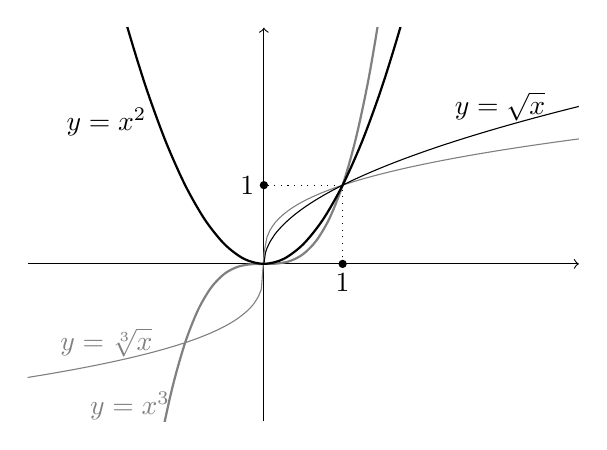
\begin{tikzpicture}[x=1.0cm,y=1.0cm]
      \clip(-3,-2) rectangle (4,3);
    	\draw[->] (-3,0) -- (4,0);
      \draw[->] (0,-2) -- (0,3);
      \draw[dotted] (1,0) -- (1,1) -- (0,1);
%      \draw[domain=0.2:4,samples=50,variable=\x,dashed,color=gray] plot
%        ({\x}, {1/(\x))});
%      \draw[domain=-3:-0.5,samples=50,variable=\x,dashed,color=gray] plot
%        ({\x}, {1/(\x))});
      \draw[domain=-2.0:2.0,smooth,variable=\x,thick,color=gray] plot
        ({\x}, {\x*\x*\x)});
      \draw[domain=-3.1:4.0,samples=200,variable=\x,color=gray] plot
        ({\x}, {pow(abs(\x),1/3)*\x / abs(\x)});
      \draw[domain=-3.0:3.0,smooth,variable=\x,thick] plot
        ({\x}, {\x*\x});
      \draw[domain=0.0:4.0,samples=200,variable=\x] plot
      ({\x}, {pow(\x,1/2)});
      \node at (-2.0,1.8) {$y=x^2$};
      \node at (3,2) {$y=\sqrt{x}$};
      \node[color=gray] at (-1.7,-1.8) {$y=x^{3}$};
      \node[color=gray] at (-2.0,-1) {$y=\sqrt[3]{x}$};
      \fill (1,0) node[below]{$1$} circle[radius=1.5pt];
      \fill (0,1) node[left]{$1$} circle[radius=1.5pt];
    \end{tikzpicture}
  \end{center}
  \caption{Grafici delle potenze $x^2$, $x^3$ e radici
  $\sqrt x$, $\sqrt[3] x$.}
  \label{fig:potenza_intera_radice}
\end{figure}

%\subsubsection{numeri irrazionali}
%
%
%Abbiamo quindi dimostrato che $\QQ$ non può essere continuo (altrimenti 
%sarebbe isomorfo a $\RR$ dove l'equazione $x^2=2$ ha soluzione). 
%Utilizzando l'irrazionalità di $\sqrt 2$ 
%possiamo ora esibire un esempio di sottoinsiemi di $\QQ$ che sono 
%\emph{separati} (nel senso della definizione~\ref{def:ordinamento_continuo})
%ma non hanno elemento di separazione in $\QQ$:
%\[
%A= \ENCLOSE{x\in\QQ\colon x^2< 2},
%\qquad
%B = \ENCLOSE{x\in \QQ\colon x<0, x^2>2}.  
%\]
%Chiaramente $A\le B$ ma in $\RR$ questi due insiemi 
%hanno come unico elemento di separazione $\sqrt 2$ che non è elemento di
%$\QQ$.
%
%% Abbiamo appena verificato che esistono numeri irrazionali. 
%% Può però essere sorprendente scoprire che non solo i numeri irrazionali 
%% sono infiniti (chiaramente se $x$ è irrazionale anche $n\cdot x$ è irrazionale 
%% se $n$ è intero o razionale) ma addirittura la cardinalità 
%% dei numeri irrazionali è maggiore di quella dei numeri razionali 
%% $\# (\RR\setminus \QQ) > \# \QQ$ (teorema~\ref{th:cantor_secondo}).
%
%Ogni numero razionale ha una rappresentazione finita. 
%Se $x=\frac p q$ possiamo scrivere $p$ e $q$ nella loro rappresentazione 
%decimale utilizzando una sequenza finita di cifre.
%Possiamo dare \emph{un nome} anche a molti
%numeri irrazionali. 
%Ad esempio $\sqrt 2$, $e$, $\pi$, $\sin 1$, $\ln 2$ identificheranno 
%alcuni numeri irrazionali. 
%Ma non è possibile dare una rappresentazione \emph{finita} di ogni numero reale.
%Per questo motivo è rilevante il fatto che i numeri razionali siano \emph{densi}
%nei numeri reali perché questo significa che ogni numero reale può essere 
%approssimato, con un errore piccolo a piacere, tramite un numero razionale.
%
\begin{theorem}[densità di $\QQ$ in $\RR$]
\label{th:densita_frazioni}%
\index{densità!frazioni}%
\index{approssimazioni!decimali}%
Dati $a,b\in \RR$ se $a<b$ esiste $q\in \QQ$ tale che $a< q < b$.

Equivalentemente dato $x\in \RR$ e dato $\eps>0$ esiste $q\in \QQ$ 
tale che $\abs{x-q} < \eps$.

Inoltre la frazione $q= \frac{p}{n}$ può essere scelta 
in modo tale che il denominatore sia una potenza di $10$: $n=10^k$.
\end{theorem}
\begin{proof}
La prima parte è conseguenza della seconda perché 
dati $a<b$
se scegliamo 
$x= \frac{a+b}{2}$ ed $\eps = \frac{b-a} 2$ se 
esiste $q$ tale che $\abs{x-q}< \eps$ 
allora 
\[
   a = \frac{a+b}{2} - \eps < q < \frac{a+b}{2} + \eps = b.
\]

Per dimostrare la seconda parte dati $x$ e $\eps$ basterà scegliere 
$n\in \NN$ tale che $\frac 1 n < \eps$ (l'esistenza di $n$ è garantita 
dal teorema~\ref{th:archimede}, proprietà archimedea) e predere $q = \frac{\lfloor nx\rfloor}{n}$
cosicché, per le proprietà della parte intera, si ha:
\[
  nx-1\le \lfloor nx\rfloor \le nx 
  \qquad\text{e quindi}\qquad
  x - \frac 1 n \le q \le x
\]
da cui $0 \le x-q < \frac 1 n < \eps$ come volevamo dimostrare.

Per avere una frazione con denominatore potenza di $10$ basta osservare 
che se aumentiamo $n$ la precisione della approssimazione aumenta. 
Dunque basta osservare che per ogni $n\in \NN$ esiste $d\in \NN$
tale che $10^d \ge n$ (basta scegliere $d=n$ e dimostrare per induzione 
che $10^n\ge n$).
\end{proof}

\begin{exercise}\label{ex:densita_irrazionali}
  Dimostrare che anche gli irrazionali 
  sono densi in $\RR$ cioè che se $a<b$ allora esiste 
  $x \in \openinterval{a}{b}$, $x\not \in \QQ$.
\end{exercise}

\subsubsection{frazioni decimali}
%
Le frazioni il cui denominatore è una potenza
di $10$ si chiamano frazioni decimali:
\[
  x = \frac{p}{10^d}, \qquad p\in \ZZ, d\in \NN.
\]
Tali frazioni si possono rappresentare
scrivendo il numero
intero $p$ e segnando un punto
\mynote{%
in Italia si preferisce utilizzare la virgola, ma
ci rassegnamo alla notazione anglosassone che ormai è
ubiqua in tutta la strumentazione elettronica.
}%
di separazione
prima della $d$-esima cifra a partire da destra.
Ad esempio scriveremo:
\[
  1.4142 = \frac{14142}{10^4}.
\]
In generale una frazione $\frac{p}{q}\in \QQ$
può essere scritta in forma decimale solamente
se, quando ridotta ai minimi termini,
risulta che $q$ non ha fattori primi diversi
da $2$ e $5$ (in quanto le potenze di dieci
hanno solo questi fattori).

Anche se non tutte le frazioni hanno una rappresentazione 
decimale finita, in ogni caso le frazioni decimali 
sono dense in $\RR$ (come dimostrato nel teorema~\ref{th:densita_frazioni})
e quindi ogni numero reale può essere approssimato, con errore piccolo a piacere,
mediante una frazione decimale.

Scriveremo
\mymargin{$\approx$}%
\index{$\approx$}%
\[
  x \approx \frac{p}{10^d}
\]
(si può leggere: ``$x$ è approssimativamente uguale a\dots'')
se
\[
    \frac{p-1}{10^d} < x < \frac{p+1}{10^d}.
\]

Ad esempio possiamo scrivere
\[
  \sqrt 2 \approx 1.41 = \frac{141}{10^2}
\]
per intendere%
\mynote{%
Si osservi che in base alla definizione data sarebbe anche corretto 
scrivere $\sqrt 2 \approx 1.42$ che però è una approssimazione 
peggiore. 
Questa ambiguità è necessaria se vogliamo evitare i casi 
limite in cui bisogna conoscere molte più cifre decimali di quelle richieste 
per capire qual è la migliore approssimazione.
}%
\begin{equation}\label{eq:approx_sqrt2}
\frac{140}{100} < \sqrt 2 < \frac{142}{100}.
\end{equation}
Nel calcolo numerico scientifico ogni uguaglianza numerica è intesa nel 
senso precedente, se non specificato diversamente. 

\begin{exercise}
Dimostrare \ref{eq:approx_sqrt2} senza 
utilizzare la calcolatrice.
\end{exercise}

Osserviamo infine che anche i calcolatori utilizzano una rappresentazione frazionaria, 
nel caso specifico \emph{binaria}, dei numeri.
I numeri frazionari su cui opera un calcolatore sono tutti della forma $\frac{p}{2^d}$.
Visto che $2$ divide $10$, le frazioni binarie sono anche sempre frazioni decimali, 
in particolare anche questi numeri sono densi in $\RR$.
\mynote{In un moderno calcolatore a 64 bit la rappresentazione binaria (float64) 
utilizza frazioni binarie con esponente $d\le 1024$. 
Questo permette di rappresentare numeri con una precisione non superiore alle 
$308$ cifre decimali. 
La rappresentazione è a virgola mobile e quindi questa precisione si può raggiungere 
solamente con numeri vicini allo zero, per numeri vicini a $1$ 
si ha invece $d\le 53$ che corrisponde ad una precisione di quasi $16$ cifre decimali.}

\subsubsection{frazioni decimali periodiche}

Le frazioni non decimali si possono scrivere con uno sviluppo
decimale \emph{periodico}. 
Non useremo mai questa notazione
che ricordiamo solamente con un esempio.
Il numero
\[
  x = 12.34\overline{567}
    = 12.34567\overline{567}
\]
è la frazione $x$ che risolve l'equazione
\[
  \frac{100x - 1234}{1000}
  = 100x-1234.567
  \qquad
\enclose
{\frac{0.\overline{567}}{1000}
= 0.000\overline{567} }
\]
ovvero
\[
  1234567 - 1234 = 99900 \cdot x,
  \qquad x = \frac{1234567-1234}{99900}.
\]

\begin{exercise}
Si verifichi che $0.\overline 9 = 1$.
\end{exercise}
    
Per passare dalla rappresentazione frazionaria alla rappresentazione 
decimale periodica basta svolgere la divisione in colonna.
Se l'algoritmo termina la frazione era decimale, altrimenti l'algoritmo 
diventa periodico e le cifre decimali si ripetono indefinitamente.


\subsection{punti all'infinito}
\label{sec:reali_estesi}
%%%%%%%%%%%%%%%%%%%
%%%%%%%%%%%%%%%%%%%
%%%%%%%%%%%%%%%%%%%

\begin{definition}[reali estesi]
\mymargin{$\bar\RR$}%
\index{$\bar{\RR}$}
Denotiamo con $\bar \RR=\RR \cup \ENCLOSE{+\infty, -\infty}$ l'insieme dei numeri reali
\mymargin{$+\infty$, $-\infty$}%
\index{$+\infty$, $-\infty$}
a cui vengono aggiunti due ulteriori \emph{quantità} che chiameremo
\emph{infinite} e che denotiamo con $+\infty$ e $-\infty$.
Diremo che $x\in \bar \RR$ è \emph{finito} se $x\in \RR$.
\end{definition}


Estendiamo la relazione d'ordine imponendo che valga
\[
  -\infty \le x \le +\infty, \qquad \forall x \in \bar\RR.
\]

Estendiamo anche la addizione e moltiplicazione
tra reali estesi imponendo che valga per ogni $x\in \bar \RR$
\begin{gather*}
  x + (+\infty) = +\infty, \qquad \text{se $x\neq -\infty$}\\
  x + (-\infty) = -\infty, \qquad \text{se $x\neq +\infty$}\\
  x \cdot (+\infty) = +\infty, \qquad
  x \cdot (-\infty) = -\infty, \qquad \text{se $x>0$} \\
  x \cdot (+\infty) = -\infty, \qquad
  x \cdot (-\infty) = +\infty, \qquad \text{se $x<0$}.
\end{gather*}

Si definiscono anche:
\[
 -(+\infty) = -\infty, \qquad
 -(-\infty) = +\infty, \qquad
 \frac{1}{+\infty} = \frac{1}{-\infty}=0
\]
facendo però attenzione che
questi formalmente non sono \emph{opposto}
e \emph{reciproco} in quanto
su $\bar \RR$ non sono più garantite
le regole: $x + (-x) = 0$ e $x \cdot (1/x) = 1$.
Infatti
le operazioni $(+\infty) + (-\infty)$ e $+\infty \cdot 0$ vengono
lasciate indefinite.

Definiamo anche il valore assoluto: $\abs{+\infty} = \abs{-\infty} = +\infty$.

Possiamo infine definire la sottrazione e la divisione tramite
addizione e moltiplicazione:
\[
  x - y = x + (-y), \qquad \frac{x}{y} = x \cdot \frac{1}{y}.
\]

Osserviamo che rispetto all'ordinamento di $\bar \RR$ tutti 
i sottoinsiemi sono limitati in quanto $+\infty = \max \bar \RR$ e  
$-\infty = \min \bar \RR$.
Dunque se diciamo che $A\subset \RR \subset \bar \RR$ è limitato 
(o illimitato) stiamo sempre facendo riferimento all'ordinamento di $\RR$ 
per il semplice fatto che la limitatezza in $\bar \RR$ è banale.
Diremo quindi sempre che $\NN$ è superiormente illimitato anche se
in $\bar \RR$ esiste il maggiorante $+\infty$.

D'altro canto è utile osservare che $\bar \RR$ ha un ordinamento 
continuo, come quello di $\RR$ e dunque, per il Teorema~\ref{th:sup}
sappiamo che ogni sottoinsieme di $\bar \RR$ ha sempre 
estremo superiore ed estremo inferiore anche se è vuoto o illimitato.

Dunque è consuetudine estendere gli operatori $\sup$ e $\inf$
a tutti i sottoinsiemi di $\RR$ ponendo 
\begin{align*}
  \sup A &= +\infty \quad \text{se $A$ non è superiormente limitato},\\
  \inf A &= -\infty \quad \text{se $A$ non è inferiormente limitato},\\
  \sup \emptyset &= -\infty, \\ 
  \inf \emptyset &= +\infty.
\end{align*}

\subsection{intervalli}

\begin{definition}[intervallo]
\label{def:intervallo}%
\mymargin{intervallo}%
\index{intervallo}%
Un insieme $I\subset \bar\RR$ si dice essere un \emph{intervallo}
se contiene tutti i punti intermedi:
\[
  \text{se $x, y \in I$ e $x<z<y$ allora $z \in I$.}
\]
\end{definition}
%
\begin{theorem}[caratterizzazione intervalli di $\RR$]
Sia $I\subset \RR$ e siano $a=\inf I$, $b=\sup I$,
$a,b\in \bar \RR$,
i suoi estremi. 
Allora $I$ è un intervallo se e solo se per ogni $x$ tale 
che $a<x<b$ si ha $x\in I$
\end{theorem}
%
\begin{proof}
Supponiamo che $I$ sia un intervallo.
Se $I=\emptyset$ si ha $a>b$ e quindi nessun $c$ verifica $a<x<b$.
Supponiamo $I\neq \emptyset$ e
sia $a < x < b$.
Visto che $a$ è il massimo dei minoranti di $I$
il numero $x$ non è un minorante dunque
deve esistere $y \in I$ tale
che $y < x$. 
Analogamente dovrebbe esistere $z\in I$
con $x < z$.
Ma allora, per definizione di intervallo, anche $x\in I$.

Viceversa supponiamo di avere $y,z\in I$ e $x\in \RR$ con $y<x<z$.
Visto che $y\ge a$ e $z\le b$ si ha $a<x<b$ e dunque, per ipotesi, 
$x\in I$, come richiesto dalla definizione di intervallo.
\end{proof}

Il teorema precedente ci dice che un intervallo contiene tutti i punti intermedi 
ai propri estremi. 
Gli estremi, tuttavia, possono essere o non essere inclusi nell'intervallo.
Punti esterni agli estremi non possono invece essere elementi dell'intervallo.
Possiamo quindi caratterizzare tutti gli intervalli di $\bar \RR$
introducendo le seguenti notazioni. Dati $a,b\in \bar \RR$ con $a\le b$
tutti i possibili intervalli con estremi $a$ e $b$ sono i seguenti:
\begin{equation}\label{eq:499494}
\begin{aligned}
\closeinterval{a}{b} &= \ENCLOSE{x\in \bar \RR\colon a \le x \le b} \\
\closeopeninterval{a}{b} &= \ENCLOSE{x\in \bar \RR\colon a \le x < b} \\
\opencloseinterval{a}{b} &= \ENCLOSE{x\in \bar \RR\colon a < x \le b}\\
\openinterval{a}{b} &= \ENCLOSE{x\in \bar \RR\colon a < x < b}.
\end{aligned}
\end{equation}
Abbiamo utilizzato le parentesi quadre per indicare che gli estremi
sono inclusi e le parentesi tonde per indicare che gli estremi sono esclusi.
Osserviamo che in alcuni testi si usano le parentesi quadre rovesciate al posto
delle parentesi tonde.

Se $a>b$ potremmo definire per convenzione:
\begin{equation}\label{eq:488364}
  [a,b] = [b,a], \quad
  [a,b) = (b,a], \quad
  (a,b] = [b,a), \quad
  (a,b) = (b,a).
\end{equation}
Si faccia però attenzione che in altri testi gli intervalli con gli estremi
scambiati non vengono definiti oppure vengono considerati vuoti.

La convenzione può essere utile perché in generale se $\vec a, \vec b$ sono
elementi di uno spazio vettoriale reale $V$ allora ha senso
definire:
\begin{align*}
    [\vec a,\vec b] &= \ENCLOSE{(1-t)\vec a + t \vec b\colon t\in [0,1]},\\
    [\vec a,\vec b) &= \ENCLOSE{(1-t)\vec a + t \vec b\colon t\in [0,1)},\\
    (\vec a,\vec b] &= \ENCLOSE{(1-t)\vec a + t \vec b\colon t\in (0,1]},\\
    (\vec a,\vec b) &= \ENCLOSE{(1-t)\vec a + t \vec b\colon t\in (0,1)}.
\end{align*}
L'intervallo $[\vec a,\vec b]$ è quindi il segmento di estremi
$\vec a$ e $\vec b$ e può essere definito anche se sullo spazio
vettoriale non è dato un ordinamento.
Questo rimane coerente con la definizione~\eqref{eq:499494}
data sopra solamente se adottiamo la convenzione~\eqref{eq:488364}.

Noi considereremo per lo più intervalli di $\RR$ (non di $\bar \RR$): in tal
caso gli estremi infiniti saranno quindi sempre esclusi dall'intervallo.

\subsection{andamento del grafico di una funzione}
%
Se $f\colon A \subset \RR\to \RR$ è una funzione, un modo molto
utile di rappresentarla graficamente è quello di disegnarne il
grafico, ovvero la curva del piano cartesiano:
\[
   G_f = \ENCLOSE{(x,y)\in A\times \RR\colon y = f(x)}.
\]
Molte proprietà della funzione potranno essere riconosciute
geometricamente guardandone il grafico.

\begin{definition}[simmetrie]
Sia $f\colon A \subset \RR \to \RR$ una funzione.
Diremo che $f$ è:
\begin{enumerate}
\item \emph{pari}%
\mymargin{pari}%
\index{pari}
\index{funzione!pari}%
se $A=-A$ (significa che se $x\in A$ allora anche $-x\in A$) e
\[
  f(-x) = f(x);
\]
\item \emph{dispari}%
\mymargin{dispari}%
\index{dispari}
\index{funzione!dispari}%
se $A=-A$ e
\[
  f(-x) = -f(x);
\]
\item \emph{periodica}%
\mymargin{periodica}%
\index{periodico}
\index{funzione!periodica}%
di periodo $T$ se $A+T=A$
(significa che $x\in A \iff x+T \in A$)
e se per ogni $x\in A$ si ha
\[
  f(x+T)=f(x)
\]
\end{enumerate}
\end{definition}

Ad esempio se $n\in \ZZ$ la funzione $f(x)=x^n$
è pari se $n$ è pari ed è dispari se $n$ è dispari.
Il grafico di una funzione dispari ha una simmetria
centrale, in quanto se $(x,f(x))\in G_f$ allora
anche $(-x,-f(x)) = (-x,f(-x))\in G_f$.
Il grafico di una funzione pari ha invece una
simmetria rispetto all'asse delle ordinate $x=0$
infatti se $(x,f(x))\in G_f$ allora $(-x,f(x)) = (-x,f(-x)) \in G_f$.

La funzione $f(x) = x - \lfloor x\rfloor$ (la parte frazionaria di $x$)
è un esempio di funzione periodica di periodo $T=1$. Infatti
è chiaro che $\lfloor x+1\rfloor = \lfloor x \rfloor +1$ e quindi
$f(x+1)=f(x)$.

Si osservi che \emph{dispari}, per le funzioni, non è la negazione
di \emph{pari}.
La funzione $f(x) = x+1$ non è né pari, né dispari, né periodica
(verificare).


\begin{definition}[zeri]
  Se $f\colon A\subset \RR \to \RR$ è una funzione diremo che
  $x\in A$ è uno \emph{zero} di $f$ se $f(x)=0$.
  L'\emph{insieme degli zeri}%
\mymargin{insieme degli zeri}%
\index{insieme!degli zeri}
  \index{zero!di una funzione}%
  è quindi dato da
  \[
    f^{-1}(\ENCLOSE{0}) = \ENCLOSE{x\in \RR\colon f(x) = 0}.
  \]
\end{definition}

Abbiamo già accennato al fatto che uno dei problemi più comuni in
matematica è quello di invertire una funzione. In particolare 
dato $y\in \RR$ ci si chiede quali siano gli $x\in \RR$ 
tali che $f(x)=y$. 
Questo problema si riconduce
a trovare gli zeri della funzione $f(x)-y$ e per questo motivo 
siamo interessati allo studio degli zeri.

Riprendiamo ora la definizione~\ref{def:monotonia} (monotonia) che da ora in avanti 
potrà essere applicata alle funzioni $f\colon A \to \RR$ definite 
su un insieme $A\subset \RR$.

Dal punto di vista grafico una funzione $f$ è crescente
se preso qualunque punto $(x,f(x))$ sul grafico della funzione
e tracciati gli assi paralleli agli assi cartesiani, passanti
per il punto fissato, si osserva che il grafico della funzione
è tutto contenuto nel primo e terzo quadrante determinati
dagli assi traslati.

E' facile verificare che la funzione $f\colon [0,+\infty)\to \RR$
definita da $f(x)=x^n$
è strettamente crescente se $n$ è un intero positivo.
Se però consideriamo la funzione definita su tutto
$\RR$: $f\colon \RR \to \RR$,
$f(x)=x^n$ allora solo se $n$ è dispari la funzione rimane
strettamente crescente
(le funzioni pari non possono mai essere strettamente crescenti se
il loro dominio contiene almeno tre punti).

Se una funzione non è monotona è piuttosto comune studiare 
la monotonia della funzione ristretta a particolari intervalli: 
su alcuni intervalli la funzione (ristretta) potrà essere crescente e su altri 
intervalli potrà essere decrescente.

\begin{exercise}
Verificare che la composizione di funzioni monotone è una
funzione monotona e la composizione di funzioni strettamente
monotone è strettamente monotona.
Quando è che la funzione composta risulta crescente?
Quando decrescente?
\end{exercise}

\begin{exercise}
Si dimostri che applicando una funzione strettamente crescente ai due
membri di una equazione o disequazione (stretta o larga che sia)
si ottiene una equazione o disequazione equivalente.
Ovviamente è necessario che la funzione sia definita dove viene applicata.

Lo stesso vale per le funzioni strettamente decrescenti 
se però si cambia il verso della disequazione.
\end{exercise}

\begin{definition}[funzioni limitate, massimo/minimo]
\label{def:funzione_limitata}%
Se $f\colon A \to \RR$ è una funzione allora definiamo
l'estremo superiore di $f$ come l'estremo superiore
dell'immagine di $f$:
\[
  \sup f = \sup_{x\in A} f(x) = \sup f(A).
\]
In maniera analoga si definiscono l'estremo inferiore $\inf f$,
il massimo $\max f$ e il minimo $\min f$.

Dunque il massimo di una funzione è (se esiste) il valore massimo
che la funzione può assumere. I punti $x$ in cui
la funzione assume il valore massimo $f(x)$ vengono chiamati
\emph{punti di massimo}.
\mymargin{punto di massimo/minimo}%
\index{punto di massimo/minimo}%
\index{punto!di massimo}%
\index{punto!di minimo}%
Analogamente i punti in cui la funzione
assume il valore minimo (sempre che esistano) vengono
chiamati \emph{punti di minimo}.

Diremo che la funzione $f$ è
\emph{superiormente limitata}%
\mymargin{funzione superiormente limitata}%
\index{superiormente limitata}
se $\sup f<+\infty$
ovvero se esiste $M\in \RR$ tale che
\[
\forall x\in A \colon f(x) \le M.
\]
Diremo che la funzione $f$ è
\emph{inferiormente limitata}%
\mymargin{funzione inferiormente limitata}%
\index{inferiormente!limitato}
se $\inf f > -\infty$ ovvero se esiste $M\in \RR$ tale che
\[
 \forall x \in A \colon f(x) \ge M.
\]
Diremo che la funzione $f$ è \emph{limitata}%
\mymargin{funzione limitata}%
\index{limitata}
se è sia superiormente che inferiormente limitata ovvero
se $\sup\abs{f}<+\infty$ cioè se esiste $M\in \RR$ tale che
\[
\forall x \in A \colon \abs{f(x)}\le M.
\]
\end{definition}

Nel seguente esercizio abbiamo un esempio di funzione limitata.
\begin{exercise}
Si consideri la funzione $f\colon \RR\to\RR$
\[
 f(x) = \frac{1}{1+x^2}.
\]
Verificare che $f$ è pari, che $\max f = \sup f = 1$, che $0$ è l'unico punto di massimo,
che $\inf f = 0$ e che $\min f$ non esiste.
\end{exercise}

\subsection{funzioni lineari}

\begin{figure}
  \begin{center}
    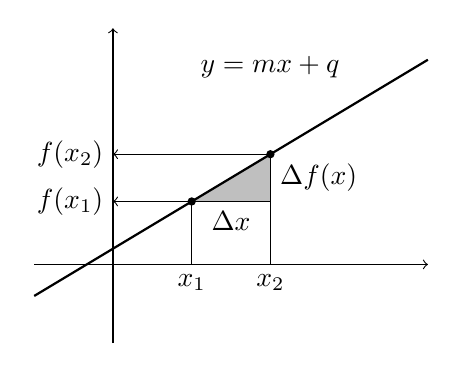
\begin{tikzpicture}[x=1.0cm,y=1.0cm]
    	\draw[->] (-1,0) -- (4,0);
      \draw[->] (0,-1) -- (0,3);
      % y = (3/5)*x + 1/5
      \fill[fill=lightgray,draw] (1,0.8) -- (2,0.8) node [midway,below]{$\Delta x$} -- (2,1.4) node [midway,right]{$\Delta f(x)$};
      \draw[thick] (-1,-0.4) -- (4,2.6);
      \draw[->] (1,0) node[below]{$x_1$} -- (1,0.8)
      -- (0,0.8) node[left]{$f(x_1)$};
      \draw[->] (2,0) node[below]{$x_2$} -- (2,1.4)
      -- (0,1.4) node[left]{$f(x_2)$};
      \fill (1,0.8) circle[radius=1.5pt];
      \fill (2,1.4) circle[radius=1.5pt];
      \node[left] at (3.0,2.5) {$y=mx+q$};
    \end{tikzpicture}
  \end{center}
  \caption{Il grafico di una funzione lineare.}
  \label{fig:funzione_lineare}
\end{figure}

Le \emph{funzioni lineari}%
\mymargin{funzione lineare}%
\index{funzioni lineari}
$f\colon \RR \to \RR$ sono le funzioni per le quali
esistono $m,q\in\RR$ tali che%
\mynote{%
Attenzione: nell'ambito dell'algebra lineare queste
funzioni verrebbero chiamate \emph{lineari affini}, mentre
le funzioni lineari dovrebbero sempre avere $q=0$.
Noi invece (come spesso accade nell'ambito dell'analisi)
chiameremo lineari queste funzioni e chiameremo
\emph{lineari omogenee} quelle con $q=0$.
Il termine \emph{lineare} pervade tutta la matematica 
e si applica in particolare alle equazioni che si ottengono 
tramite le funzioni lineari.
Purtroppo il nome scelto è fuorviante: la parola \emph{linea} viene 
usata a volte come abbreviazione di \emph{linea retta}, quando 
invece sarebbe più giusto utilizzare l'abbreviazione \emph{retta}
in quanto una linea può benissimo essere curva.
In altri contesti (come ad esempio nell'ambito degli ordinamenti)
il termine \emph{lineare} rappresenta un oggetto unidimensionale
senza ramificazioni ed è quindi maggiormente aderente 
al significato originale della parola.
} % marginnote
\[
  f(x) = mx + q.
\]

Se prendiamo due punti $(x_1,f(x_1))$
e $(x_2,f(x_2))$ sul grafico di una funzione lineare
possiamo osservare che si ha
\[
  \frac{f(x_2) - f(x_1)}{x_2 - x_1} = m.
\]
Il coefficiente $m$, dunque, rappresenta la pendenza del
grafico di $f$, ovvero il rapporto tra la variazione
dei valori della funzione $\Delta f = f(x_2) - f(x_1)$
e la variazione della variabile in ingresso
$\Delta x = x_2 - x_1$.
Geometricamente questo è il rapporto tra i due cateti
(base e altezza) che formano un triangolo rettangolo la
cui ipotenusa è il segmento che congiunge i due punti sul grafico.
Il fatto che questo rapporto sia costante significa,
in base al teorema di Talete, che i punti del grafico sono
allineati ovvero che il grafico di una funzione lineare è,
dal punto di vista geometrico, una retta.

\begin{definition}[retta]
  \index{retta}%
  \index{linea!retta}%
  Una \emph{linea retta} (più semplicemente: \emph{retta}) in uno spazio affine
  è un sottospazio affine di dimensione 1 
  ovvero la traslazione di un sottospazio vettoriale di dimensione 1
  (si rimanda al corso di geometria).
\end{definition}

Tutte le rette del piano, 
tranne quelle parallele all'asse delle ordinate,
sono grafico di una funzione lineare.

Si osservi che per $m>0$ la funzione è strettamente crescente,
per $m=0$ la funzione è costante e per $m<0$ la funzione è
strettamente decrescente.

\subsection{funzioni quadratiche}
\label{sec:funzioni_quadratiche}

\begin{figure}
  \begin{center}
    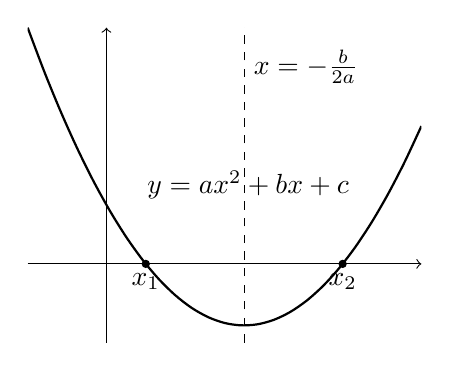
\begin{tikzpicture}[x=1.0cm,y=1.0cm]
      \clip(-1,-1) rectangle (4,3);
    	\draw[->] (-1,0) -- (4,0);
      \draw[->] (0,-1) -- (0,3);
      % y = (3/5)*x + 1/5
      \draw[dashed] (1.75,-1) -- (1.75,4);
      \node[right] at (1.75,2.5){$x=-\frac b {2a}$};
      \draw[domain=-1.0:4.0,smooth,variable=\x,thick] plot
      ({\x}, {0.5*(\x-0.5)*(\x-3.0)});
      \fill (0.5,0.0) node[below]{$x_1$} circle[radius=1.5pt];
      \fill (3,0.0) node[below]{$x_2$} circle[radius=1.5pt];
      \node at (1.8,1) {$y=ax^2+bx+c$};
    \end{tikzpicture}
  \end{center}
  \caption{Il grafico di una funzione quadratica.}
  \label{fig:funzione_quadratica}
\end{figure}

Le funzioni espresse mediante un \emph{polinomio di secondo grado}%
\mymargin{polinomio di secondo grado}%
\index{polinomio!di secondo grado}
\begin{equation}\label{eq:funzione_quadratica}
  f(x) = ax^2 + bx +c
\end{equation}
con $a,b,c\in \RR$, $a\neq 0$, si possono chiamare
\emph{funzioni quadratiche}%
\mymargin{funzioni quadratiche}%
\index{funzione!quadratica}.

Il modello di funzione quadratica è la funzione
$f(x) = x^2$ che (come tutte le potenze di esponente positivo e pari)
risulta essere una funzione pari, strettamente crescente
sull'intervallo $[0,+\infty)$ e strettamente decrescente
su $(-\infty,0]$. La funzione assume solamente valori non negativi
e si annulla solo per $x=0$.
Dunque l'equazione
\[
  x^2 = b
\]
non ha soluzione se $b<0$ ed ha come unica soluzione $x=0$ se $b=0$.
Se $b>0$ sappiamo che
questa equazione ha una unica soluzione positiva $x_1 = \sqrt{b}$
e, per simmetria, ha anche una soluzione negativa $x_2 = -\sqrt{b}$.
Sintetizzando si usa scrivere $x_{1,2} = \pm \sqrt{b}$
per condensare in una unica riga le due definizioni.

La generica funzione quadratica~\eqref{eq:funzione_quadratica}
può essere ricondotta al caso modello tramite un cambio
di variabile lineare. In pratica si cerca di comporre il quadrato
di un binomio con un procedimento chiamato
\emph{completamento del quadrato}%
\mymargin{completamento del quadrato}%
\index{completamento del quadrato}:
\begin{equation}\label{eq:24589}
\begin{aligned}
f(x) = ax^2+bx+c
  &= a \Enclose{x^2+\frac b a x + \frac c a}\\
  &= a \Enclose{x^2+2 \frac{b}{2a} x + \frac{b^2}{4a^2} - \frac{b^2}{4a^2} + \frac c a}\\
  &= a \Enclose{\enclose{x+\frac{b}{2a}}^2 - \frac{b^2-4ac}{4a^2}} \\
  &= a\enclose{x+\frac b{2a}}^2  - \frac{b^2-4ac}{4a}.
\end{aligned}
\end{equation}

Ponendo $X=x+\frac b{2a}$ e $Y=y+\frac{b^2-4ac}{4a}$
l'equazione $y=ax^2+bx+c$ diventa quindi $Y=aX^2$. 
Significa
che il grafico della funzione quadratica~\eqref{eq:funzione_quadratica}
si ottiene traslando la curva $y = a x^2$ che, 
dal punto di vista geometrico, si può facilmente
dimostrare essere una parabola con fuoco
nel punto di coordinate $\enclose{0,\frac 1 {4a}}$
e asse la retta di equazione $x=0$.
Dunque il grafico di ogni funzione quadratica è una parabola, 
e più precisamente: ogni parabola con direttrice parallela all'asse delle
ascisse è il grafico di una funzione quadratica.

\begin{definition}[parabola]
  \index{parabola}%
  \index{fuoco!parabola}%
  \index{direttrice!parabola}%
  La parabola $P_{\vec F,r}$ con \emph{fuoco} nel punto $\vec F=(F_1,F_2)\in \RR\times \RR$ 
  e retta \emph{direttrice}
  la retta $r \subset \RR\times\RR$ 
  è l'insieme dei punti  $\vec x = (x_1,x_2)\in \RR\times\RR$ 
  equidistanti da $\vec F$ e da $r$:
  \[
  P_{\vec F,r} = \ENCLOSE{\vec x\in \RR\times\RR\colon 
  \sqrt{(x_1-F_1)^2 + (x_2-F_2)^2} 
  = \inf_{\vec P\in r}\sqrt{(x_1-P_1)^2+(y_1-P_1)^2}
  }.
  \]
\end{definition}

\begin{exercise}
  Si dimostri che per ogni $a\neq 0$ esiste $s\neq 0$ 
  per cui il riscalamento $X=sx$, $Y=sy$ porta il grafico della 
  parabola $y=ax^2$ nel grafico della parabola $Y=X^2$.
  Significa che 
  c'è una unica parabola 
  a meno di isometrie e riscalamenti.
\end{exercise}

Ricordando le proprietà di monotonia della funzione $X\mapsto X^2$
possiamo dedurre che se $a>0$ la funzione $f(x)$ è strettamente
decrescente se ristretta all'intervallo 
$\left(-\infty,-\frac b {2a}\right]$ ed è invece strettamente crescente 
sull'intervallo $\left[-\frac b{2a},+\infty\right)$. 
Ha dunque un punto di minimo in $x=-\frac{b}{2a}$.
Inoltre (sempre se $a>0$) la funzione è superiormente illimitata.
Viceversa se $a<0$ la funzione è inferiormente illimitata ed ha 
un massimo nel punto $x=-\frac{b}{2a}$.

E' molto importante saper risolvere equazioni e disequazioni
quadratiche. Grazie a~\eqref{eq:24589} l'equazione
\[
 a x^2 + bx + c = 0
\]
risulta equivalente a
\[
  \enclose{x+\frac{b}{2a}}^2 = \frac{b^2-4ac}{4a^2}.
\]
Dunque se $b^2-4ac<0$ l'equazione $ax^2+bx+c=0$ non ha soluzioni.
Se $b^2-4ac=0$ l'equazione ha una unica soluzione $x=-\frac{b}{2a}$.
Infine se $b^2-4ac>0$ si ottiene
\[
  x+\frac b{2a} = \pm \frac{\sqrt{b^2-4ac}}{2a}
\]
da cui la famosa formula risolutiva
\mymark{***}
\begin{equation}\label{eq:secondo_grado}
  x_{1,2} = \frac{-b \pm \sqrt{b^2-4ac}}{2a}.
\end{equation}

Risolvendo le disequazioni allo stesso modo, si trova
che la funzione $ax^2+bx+c$, quando $a>0$ è positiva
nei punti esterni alle soluzioni dell'equazione
(in tutti i punti se le soluzioni non esistono) ed
è negativa nei punti interni alle due soluzioni.
Viceversa se $a<0$ la funzione è positiva all'interno
delle due soluzioni e negativa all'esterno.


\subsection{funzioni esponenziali}
%
%
\label{sec:esponenziale}%

Il teorema di isomorfismo ci ha permesso di definire la moltiplicazione sui 
numeri reali. 
Lo stesso identico metodo ci permetterà di definire la funzione esponenziale
ovvero la potenza $a^x$ con base $a>0$ fissata ed esponente variabile $x\in \RR$.
Abbiamo infatti già osservato che l'insieme $\RR_+$ dei reali positivi
risulta essere un gruppo moltiplicativo totalmente ordinato, denso e continuo 
(teorema~\ref{th:gruppo_moltiplicativo}).

\begin{theorem}[funzione esponenziale]
  \label{th:esponenziale}%
Dato $a\in \RR$, $a\ge 1$ per ogni $x\in \RR$ si può definire in modo unico 
la funzione esponenziale $x\mapsto a^x$ con le seguenti proprietà:
\begin{enumerate}
  \item $a^1=a$;
  \item $a^{x+y} = a^x \cdot a^y$;
  \item $a^x\ge 1$ se $x\ge 0$.
\end{enumerate}
Se $0<a \le 1$ si può definire in modo unico l'esponenziale $x\mapsto a^x$ 
con le stesse proprietà, salvo che per ogni $x\ge 0$ si ha $a^x\le 1$.

Inoltre l'esponenziale ha le seguenti proprietà, 
valide per $a,b>0$, $x,y\in \RR$:
\begin{enumerate}
  \item $a^0=1$;
  \item $a^{-1} = \frac{1}{a}$;
  \item $(a\cdot b)^x = a^x\cdot b^x$;
  \item $(a^x)^y = a^{x\cdot y}$;
  \item $a^x \le a^y$ se $a\ge 1$ e $x\le y$;
  \item $1^x=1$.
\end{enumerate}
\end{theorem}
%
\begin{proof}
Fissato $a>0$ possiamo applicare il teorema~\ref{th:isomorfismo} (isomorfismo)
con $R=\RR$ gruppo additivo e $S=\RR_+$ gruppo moltiplicativo.
Se $a\ge 1$ si ottiene l'esistenza di una, unica, funzione $\phi_a\colon \RR \to \RR_+$ 
che soddisfa le seguenti proprietà:
$\phi_a(1)=a$, $\phi_a(x+y) = \phi_a(x)\cdot \phi_a(y)$, 
$\phi_a(x)\ge 1$ se $x\ge 0$. 
Se $0<a\le 1$ otteniamo una unica funzione con le stesse proprietà 
ma $\phi_a(x) \le 1$ se $x\ge 0$.

Definiamo $a^x = \phi_a(x)$ e la chiamiamo \emph{funzione esponenziale}
con \emph{base} $a>0$ ed esponente $x\in \RR$.
  
L'omomorfismo manda sempre l'elemento neutro nell'elemento 
neutro dunque $a^0 = 1$.
\mynote{Ricordiamo che in partenza abbiamo il gruppo additivo $\RR$
con elemento neutro $0$ mentre in arrivo 
abbiamo il gruppo moltiplicativo $\RR_+$ con elemento neutro $1$.}

\mymargin{$a^{-1}=\frac 1 a$}
Per la proprietà di omomorfismo si ha $a^{x-x} = a^x \cdot a^{-x}$
da cui $a^{-x}$ risulta essere il reciproco di $a^x$ cioè 
$a^{-x}= 1/a^x$.

Per la potenza del prodotto fissati $a,b\ge 1$ basta considerare la 
funzione $f(x) = a^x\cdot b^x$. 
\mymargin{$(a\cdot b)^x = a^x\cdot b^x$}
Chiaramente $f$ è un omomorfismo in quanto $a^x$ e $a^y$ lo sono 
(e il prodotto è commutativo): 
$a^{x+y}\cdot b^{x+y} = a^x \cdot b^x\cdot a^yb^y$.
Inoltre se $x\ge 0$ si ha $a^x\ge1$ e $b^x\ge 1$ da cui $f_(x)\ge 1$.
Essendo $f(1) = a^1\cdot b^1 = a\cdot b$ 
per l'unicità dell'omomorfismo positivo concludiamo che $f = \phi_{a\cdot b}$
cioè $a^x\cdot b^x = (a\cdot b)^x$.
Usando la regola del reciproco possiamo estendere questa proprietà 
quando $a<1$ e/o $b<1$ (ma sempre $a,b\ge 0$).

\mymargin{$(a^x)^y = a^{x\cdot y}$}
Infine per la potenza di potenza fissato $a\ge 1$ e $x\ge 0$ 
consideriamo la funzione $f(y) = a^{x\cdot y}$.
Per le proprietà precedenti si verifica facilmente che  
$f(y+z) = f(x)\cdot f(z)$. 
Inoltre se $a\ge 1$, $x\ge 0$ e $y\ge 0$ si ha 
$f(y)\ge 1$ che è la positività. 
Dunque per il teorema di isomorfismo,
essendo $f(1)=a^x$, si ottiene $f(y) = (a^x)^y$
che è quanto volevamo dimostrare.
La regola del reciproco estende questa proprietà 
ai casi $x\le 0$ e $a\le 1$ (sempre con $a\ge 0$).

Se $a\ge 1$ e $x\le y$ allora $a^{y-x}\ge 1$.
\mymargin{monotonia}
Ma $a^{y-x} = \frac{a^y}{a^x}$ e dunque $a^y\ge a^x$.

Se $a=1$ per $x\ge 0$ si ha contemporaneamente $1^x\ge 1$ e $1^x\le 1$
dunque $1^x=1$. 
Lo stesso vale se $x\le 0$ in quanto $1^{-x}=\frac 1{1^x}$.
\mymargin{$1^x=1$}
\end{proof}

\begin{figure}
  \begin{center}
    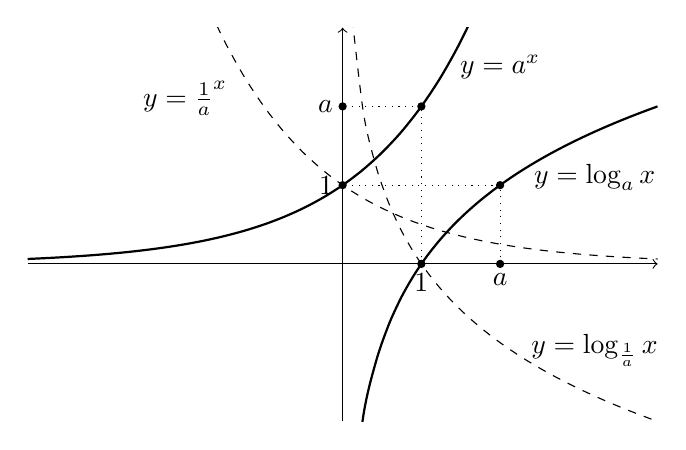
\begin{tikzpicture}[x=1.0cm,y=1.0cm]
      \clip(-4,-2) rectangle (4,3);
    	\draw[->] (-4,0) -- (4,0);
      \draw[->] (0,-2) -- (0,3);
      % y = (3/5)*x + 1/5
      \draw[dotted] (1,0) -- (1,2) -- (0,2);
      \draw[dotted] (2,0) -- (2,1) -- (0,1);
%      \node[right] at (1.75,2.5){$x=-\frac b {2a}$};
      \draw[domain=-2.0:4.0,smooth,variable=\x,dashed] plot
        ({\x}, {pow(2,-\x)});
      \draw[domain=0.1:4.0,smooth,variable=\x,dashed] plot
        ({\x}, {-ln(\x) / ln(2)});
      \draw[domain=-4.0:2.0,smooth,variable=\x,thick] plot
        ({\x}, {pow(2,\x)});
      \node at (2,2.5) {$y=a^x$};
      \node at (-2,2.1) {$y=\enclose{\frac 1 a}^x$};
      \fill (0,1.0) node[left]{\!\!$1$} circle[radius=1.5pt];
      \draw[domain=0.1:4.0,smooth,variable=\x,thick] plot
        ({\x}, {ln(\x) / ln(2)});
      \node at (3.2,1.1) {$y=\log_a x$};
      \node at (3.2,-1.1) {$y=\log_{\frac 1 a} x$};
      \fill (1,0) node[below]{$1$} circle[radius=1.5pt];
      \fill (0,2) node[left]{$a$} circle[radius=1.5pt];
      \fill (2,0) node[below]{$a$} circle[radius=1.5pt];
      \fill (2,1) circle[radius=1.5pt];
      \fill (1,2) circle[radius=1.5pt];
    \end{tikzpicture}
  \end{center}
  \caption{Il grafico della funzione esponenziale e logaritmo 
  in base $a>1$ e $\frac 1 a < 1$ ($a=2$ in figura).}
  \label{fig:esponenziale_logaritmo}
\end{figure}




%
\subsection{logaritmo}
%
%
%

\label{sec:logaritmo}
\index{logaritmo}%

Il teorema di isomorfismo ci dice che fissato $a\in \RR_+$, $a\neq 1$ 
la funzione $\phi_a\colon \RR\to\RR_+$ definita nel paragrafo 
precedente ($\phi_a(x)=a^x$) è bigettiva.
La funzione inversa si chiama \emph{logaritmo in base $a$}
e si denota con $\log_a\colon \RR_+ \to \RR$.

Grazie alle proprietà della funzione esponenziale, già dimostrate
nel teorema~\ref{th:esponenziale} possiamo ottenere 
le proprietà del logaritmo.

\begin{theorem}[proprietà del logaritmo]
Per ogni $a>1$
esiste una unica funzione $\log_a\colon \RR_+\to \RR$ 
tale che 
\begin{enumerate}
  \item $\log_a(a) = 1$;
  \item $\log_a(x\cdot y) =\log_a x + \log_a y$;
  \item $\log_a x \ge 0$ se $x\ge 1$. 
\end{enumerate}
Se $0<a<1$ 
esiste una unica funzione $\log_a$ con le stesse proprietà 
salvo che $\log_a x \le 0$ se $x\ge 1$.

La funzione $\log_a$ viene chiamata \emph{logaritmo in base $a$}
ed ha inoltre le seguenti proprietà valide 
per ogni $a>0$, $a\neq 1$, $x,y\in \RR$, $b>0$, $c>0$, $c\neq 1$:
\begin{enumerate}
  \item $\log_a x = y$ se e solo se $a^y = x$;
  \item $\log_a 1 = 0$;
  \item $\log_a (b^x) = x\log_a b$;
  \item $\log_a x = \frac{\log_c x}{\log_c a}$.
\end{enumerate}
\end{theorem}

\subsection{potenze con esponente reale}

Nel capitolo~\ref{sec:potenza} abbiamo definito 
la funzione potenza $x^n$ con base $x\in \RR$ 
ed esponente $n\in \NN$. 
Invertendo la fuzione $x^n$ 
(solo per $x\ge 0$ quando $n$ è pari e positivo, per ogni $x\in \RR$ se 
$n$ è dispari) abbiamo definito la radice $n$-esima 
$\sqrt[n]{x}$.
Nel capitolo~\ref{sec:esponenziale} abbiamo 
definito la funzione esponenziale $a^x$ con 
base $a\in \RR_+$ ed esponente $x\in \RR$.
La funzione inversa dell'esponenziale 
è il logaritmo $\log_a x$ definito per $x>0$.

Quando $a>0$ 
e $b\in \NN$,
abbiamo formalmente due diverse definizioni 
dell'operazione \emph{potenza} $a^b$ ma, 
ovviamente, queste due definizioni 
coincidono in quanto il teorema di isomorfismo 
ci garantisce che la funzione esponenziale 
$a^x$ coincide con la moltiplicazione ripetuta 
quando $x$ è un numero naturale.
Grazie a questa osservazione possiamo osservare 
che se $x>0$, $p\in \NN$ e $q\in \NN$, $q\neq 0$ si ha 
\begin{equation}
\label{eq:9783023}
  x^{\frac p q} = \sqrt[q]{x^p}, 
  \qquad 
  x^{-\frac p q} = \frac{1}{\sqrt[q]{x^p}}
\end{equation}
in quanto 
\[
  \enclose{x^{\frac p q}}^q = x^p,
  \qquad
  x^{-y} = \frac{1}{x^y}.
\]
Se ripercorriamo la dimostrazione del teorema di isomorfismo 
usando in arrivo il gruppo additivo (è così che abbiamo 
definito la funzione esponenziale) ci accorgiamo 
che la funzione $a^x$ viene dapprima definita sugli $x$
naturali come moltiplicazione ripetuta, 
poi sugli $x$ razionali 
positivi tramite la radice $n$-esima e poi sugli 
$x$ negativi passando al reciproco.

Senz'altro potrà essere utile definire 
$a^{-n} = \frac 1 {a^n}$ avendo quindi una definizione 
di potenza $a^n$ valida per ogni $a$ se $n\in \NN$ 
e per ogni $a\neq 0$ se $n\in \ZZ$.
In alcuni testi si va oltre e si considera $a^b$ 
definito anche quando $a<0$ e $b$ è razionale
utilizzando il lato destro delle equazioni 
in~\eqref{eq:9783023}.
Ognuno può scegliere le definizioni che preferisce 
ed è bene ricordare che le definizioni si scelgono, 
non si dimostrano. 
E' però anche bene sapere che certe definizioni 
possono essere fuorvianti.

Ci sono buoni motivi per pensare che la funzione 
esponenziale $a^x$ ($a>0$) e la funzione potenza $x^n$ 
con $n\in \NN$ siano funzioni sostanzialmente diverse.
Si noti ad esempio che le regole delle potenze sono 
soddisfatte da entrambe le definizioni, separatamente, 
ma se mescoliamo le due definizioni le proprietà 
possono cadere. Ad esempio:
\[
  \enclose{(-2)^6}^{\frac 1 2} 
  \neq \enclose{-2}^{6\cdot \frac 1 2}.
\]

Anche il fatto che abbiamo definito $0^0=1$ andrebbe 
interpretato nel senso che lo $0$ all'esponente 
è un numero naturale, non un numero reale:
La funzione esponenziale $a^x$ è definita 
solo per $a>0$ mentre la funzione $x^n$ è definita anche 
per $x=0$ ma solo per $n\in \NN$.


% \begin{figure}
%   \begin{center}
%     \begin{tikzpicture}[x=1.0cm,y=1.0cm]
%       \clip(-3,-2) rectangle (4,3);
%     	\draw[->] (-3,0) -- (4,0);
%       \draw[->] (0,-2) -- (0,3);
%       \draw[dotted] (1,0) -- (1,1) -- (0,1);
%       % \draw[dotted] (2,0) -- (2,1) -- (0,1);
%       \draw[domain=0.5:4,samples=50,variable=\x,thick,dashed] plot
%         ({\x}, {1/(\x*\x))});
%       \draw[domain=-3:-0.5,samples=50,variable=\x,thick,dashed] plot
%         ({\x}, {1/(\x*\x))});
%       \draw[domain=0.2:4,samples=50,variable=\x,dashed,color=gray] plot
%         ({\x}, {1/(\x))});
%       \draw[domain=-3:-0.5,samples=50,variable=\x,dashed,color=gray] plot
%         ({\x}, {1/(\x))});
%       \draw[domain=-2.0:2.0,smooth,variable=\x,thick,color=gray] plot
%         ({\x}, {\x*\x*\x)});
%       \draw[domain=-3.1:4.0,samples=200,variable=\x,color=gray] plot
%         ({\x}, {pow(abs(\x),1/3)*\x / abs(\x)});
%       \draw[domain=-3.0:3.0,smooth,variable=\x,thick] plot
%         ({\x}, {\x*\x});
%       \draw[domain=0.0:4.0,samples=200,variable=\x] plot
%       ({\x}, {pow(\x,1/2)});
%       \node at (-2.0,1.8) {$y=x^2$};
%       \node at (3,2) {$y=\sqrt{x}$};
%       \node[color=gray] at (-1.7,-1.8) {$y=x^{3}$};
%       \node[color=gray] at (-2.0,-1) {$y=\sqrt[3]{x}$};
%       \node[color=gray] at (-1.7,-0.3) {$y=\frac 1 x$};
%       \node at (-2.5,0.6) {$y=\frac 1 {x^2}$};
%       \fill (1,0) node[below]{$1$} circle[radius=1.5pt];
%       \fill (0,1) node[left]{$1$} circle[radius=1.5pt];
%     \end{tikzpicture}
%   \end{center}
%   \caption{Grafici tipici di potenze e radici.}
%   \label{fig:potenza_radice}
% \end{figure}


\subsection{equazioni e disequazioni}

Un problema matematico molto comune è quello di dover risolvere 
equazioni e disequazioni del tipo:
\begin{equation}\label{eq:573197}
  f(x) = b, \quad f(x) \ge b, \quad f(x) > b, 
  \quad f(x) \le b, \quad f(x) < b
\end{equation}
dove $f\colon A \subset \RR \to\RR$ è una funzione data e 
$b\in \RR$ è fissato.

Quando $f$ è strettamente crescente e $b\in f(A)$ 
la soluzione può essere 
scritta banalmente: 
ovviamente deve essere $x\in A$
e ogni equazione o disequazione in~\eqref{eq:573197}
avrà la corrispondente soluzione:
\[
  x= f^{-1}(b), \quad x \ge f^{-1}(b), \quad x>f^{-1}(b),
  \quad x \le f^{-1}(b), \quad x < f^{-1}(b).
\]
Se la funzione fosse strettamente decrescente 
si può procedere allo stesso modo, ma le disuguaglianze si invertono.
Se la funzione fosse strettamente crescente su alcuni intervalli 
e strettamente decrescente su altri si potranno separare i diversi 
casi e si otterranno più soluzioni espresse da uguaglianze
o disuguaglianze.

\begin{example}
  Si risolva la disequazione 
  \[
   \log_2\Enclose{\sqrt[3]{(x+1)^4-3}-2} \le 3. 
  \]
\end{example}%
\begin{proof}[Svolgimento.]
La funzione logaritmo è strettamente crescente ed è definita 
quando l'argomento è positivo. 
Dunque la disequazione data 
è equivalente al sistema di disequazioni:
\[
0 < \sqrt[3]{(x+1)^4 - 3} - 2 \le 8.  
\]
Possiamo sommare $2$ per ottenere 
\[
  2 < \sqrt[3]{(x+1)^4 - 3} \le 10.  
\]
La funzione radice cubica è strettamente crescente 
su tutto $\RR$ quindi possiamo invertirla elevando 
tutto al cubo:
\[
 8 < (x+1)^4 - 3 \le 1000.
\]
Sommiamo $3$:
\[
11 < (x+1)^4 \le 1003.  
\]
L'elevamento alla quarta potenza è strettamente crescente 
solo quando l'argomento è positivo, ed è una funzione pari.
Possiamo quindi affermare che le nostre disequazioni sono 
equivalenti all'unione delle soluzioni di due sistemi:
\[
  \sqrt[4]{11} < x+1 \le \sqrt[4]{1003}
  \qquad\text{o}\qquad 
  -\sqrt[4]{1003} \le x+1 < -\sqrt[4]{11}.
\]
Sottraendo $1$ otteniamo infine 
\[
  \sqrt[4]{11} -1 < x \le \sqrt[4]{1003} - 1
  \qquad\text{o}\qquad 
  -\sqrt[4]{1003} -1 \le x < -\sqrt[4]{11} -1.
\]
In definitiva l'insieme delle soluzioni è 
\[
\left[-\sqrt[4]{1003} - 1, -\sqrt[4]{11}-1\right)
\cup \left(\sqrt[4]{11}-1 , \sqrt[4]{1003} -1\right].  
\]
\end{proof}

Nell'esempio precedente la funzione 
$f(x) = \log_2\Enclose{\sqrt[3]{(x+1)^4-3}-2}$
è ottenuta mediante composizione di funzioni elementari:
\begin{align*}
f &= (x\mapsto \log_2 x)\circ(x\mapsto x-2)\circ (x \mapsto \sqrt[3]{x})\\
  &\quad \circ (x \mapsto x-3) \circ (x\mapsto x^4) \circ (x\mapsto x+1).
\end{align*}
Negli intervalli in cui tutte queste funzioni sono invertibili 
la funzione inversa si ottiene componendo, in ordine opposto,
tutte le inverse:
\begin{align*}
  f^{-1} &= (x\mapsto x-1) \circ (x\mapsto \sqrt[4]{x}) \circ (x \mapsto x+3) \\
    &\quad \circ (x \mapsto x^3) \circ (x \mapsto x+2) \circ (x\mapsto 2^x).
\end{align*}
In effetti il caposaldo $\sqrt[4]{1003}-1$ è proprio tale 
funzione valutata in $b=3$.

Il metodo precedente è puramente algebrico e 
si applica alle equazioni 
come la~\eqref{eq:573197} dove la variabile $x$ 
compare una sola volta e dove la funzione $f$ si esprime 
come composizione di funzioni elementari di cui sappiamo 
scrivere la funzione inversa. 

Ben diverso è il caso in cui nell'equazione la variabile $x$ 
compare più di una volta.
In alcuni casi, come ad esempio,
\[
  x^2 > 2x - 1  
\]
queste equazioni 
possono essere ricondotte al caso precedente tramite 
opportune manipolazioni algebriche.
Il caso delle equazioni quadratiche lo abbiamo 
fatto nel paragrafo precedente utilizzato il completamento 
del quadrato: $x^2-2x = (x-1)^2-1$. 
In altri casi, come ad esempio l'equazione
\[
  2^x = x^2
\]  
le manipolazioni algebriche non sono utili.
Nel capitolo sul calcolo differenziale svilupperemo degli strumenti 
che ci permetteranno di determinare l'andamento di molte di queste 
di funzioni. 
Nel capitolo sulle successioni svilupperemo invece gli strumenti 
che ci permetteranno di determinare le soluzioni mediante 
algoritmi di approssimazione.
Questi strumenti presuppongono il concetto 
di limite e continuità: è sostanzialmente questo che identifica 
la materia chiamata analisi matematica.

